\documentclass[a4paper, 11pt, oneside, polutonikogreek, french]{article}
\usepackage{kmath, kerkis}
\usepackage[T1]{fontenc}
\usepackage{textalpha}
\usepackage{graphicx}
\usepackage{float}
\graphicspath{ {./} }
\usepackage[figurename=]{caption}
\usepackage{listings}
\usepackage{subcaption}
\lstset{basicstyle=\ttfamily}

% Babel package:
\usepackage{babel}
\usepackage{cjhebrew}
% With XeTeX/LuaTeX, load fontspec after babel to use Unicode
% fonts for Latin script and LGR for Greek:
\ifdefined\luatexversion \usepackage{fontspec}\fi
\ifdefined\XeTeXrevision \usepackage{fontspec}\fi

% "`Lipsiakos" italic font `cbleipzig`:
\newcommand*{\lishape}{\fontencoding{LGR}\fontfamily{cmr}%
		       \fontshape{li}\selectfont}
\DeclareTextFontCommand{\textli}{\lishape}
\usepackage{tocloft}
\cftsetindents{subsubsection}{3em}{7em}
\cftsetindents{subsection}{3em}{6em}
\cftsetindents{section}{3em}{6em}
\usepackage[dvipsnames]{xcolor}
\usepackage{eso-pic,graphicx}
\usepackage[top=137mm, bottom=71mm, outer=68mm, inner=68mm]{geometry}
\setlength{\columnsep}{70pt}
\color{White}
\AddToShipoutPictureBG{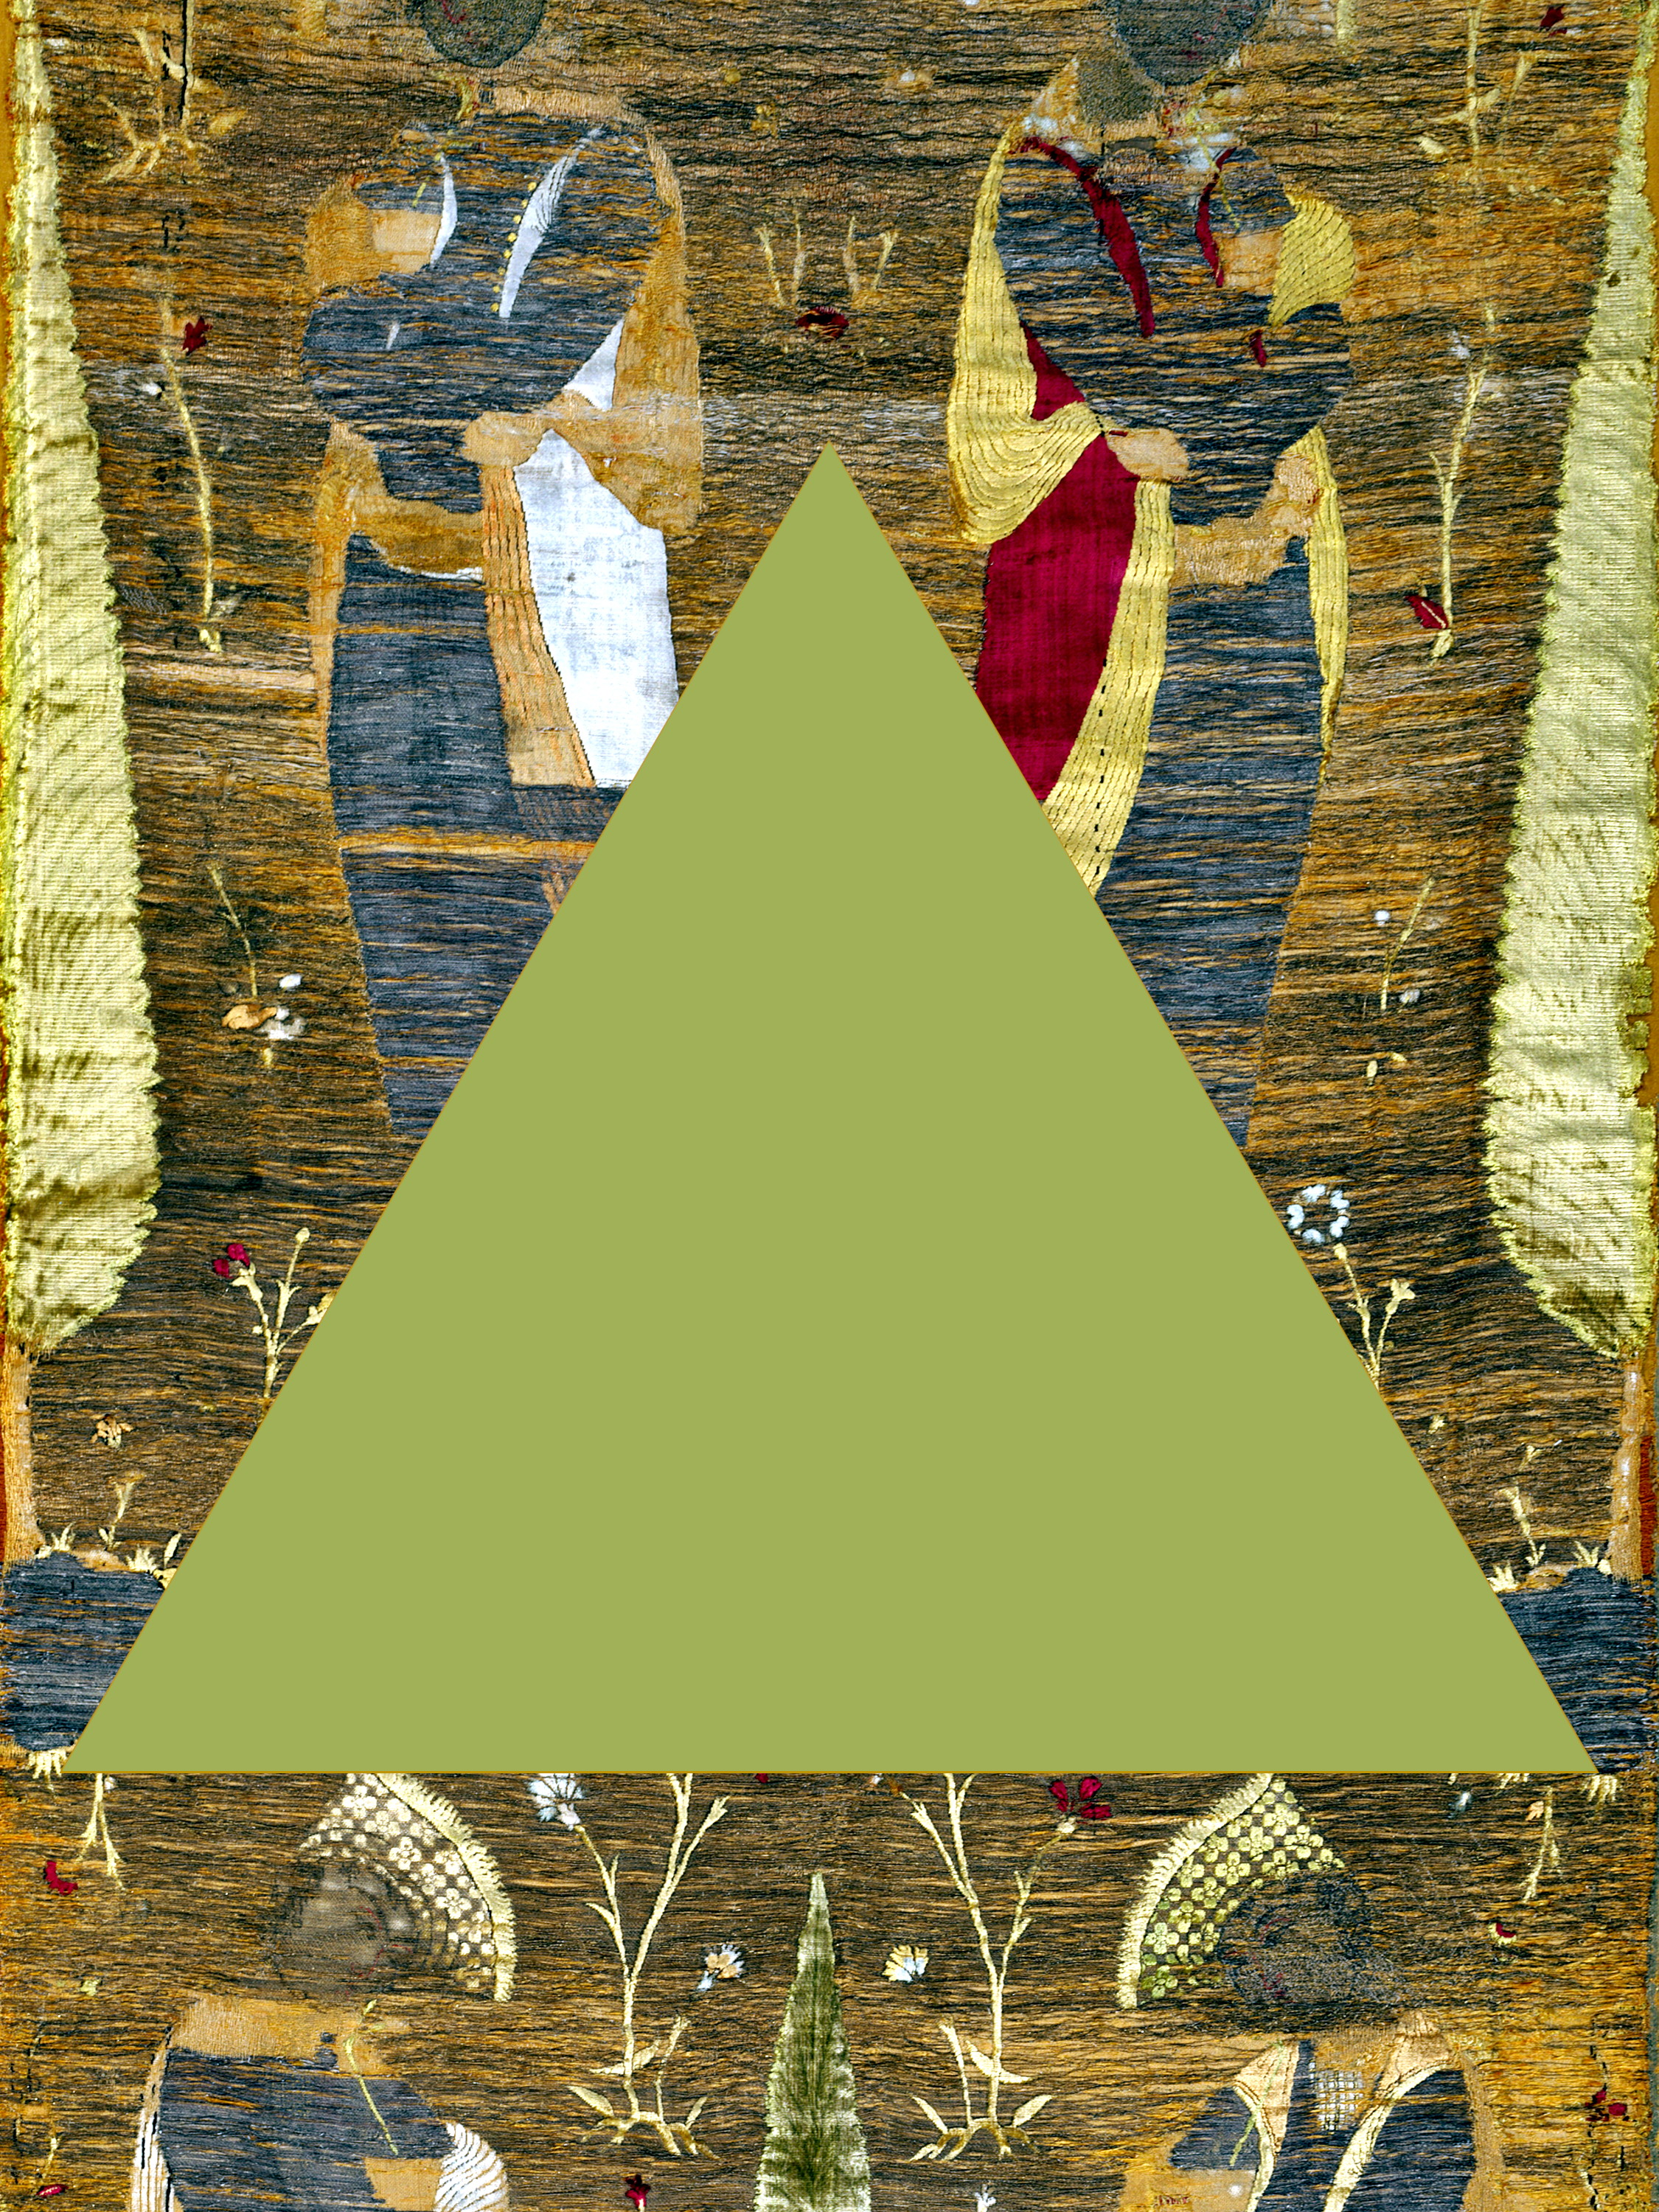
\includegraphics[width=\paperwidth,height=\paperheight]{cypress2.jpeg}}

\usepackage{svg}
\newcommand*\arabicAA{\raisebox{-0.3ex}{\includesvg[height=1em]{svg001.svg}}}
\newcommand*\arabicAB{\raisebox{-0.7ex}{\includesvg[height=1em]{svg002.svg}}}
\newcommand*\arabicAC{\raisebox{-0.5ex}{\includesvg[height=1em]{svg003.svg}}}
\usepackage{booktabs}
\setlength{\emergencystretch}{15pt}
\usepackage{microtype}
\usepackage{fancyhdr}

\begin{document}

\renewcommand\thefootnote{\tiny{\arabic{footnote}}}
\let\oldfootnote\footnote
    \renewcommand{\footnote}[1]{\oldfootnote{\bfseries\scriptsize#1}}
\bfseries
\fancypagestyle{plain}{%
\fancyhf{} % clear all header and footer fields
\fancyfoot[C]{\bfseries\tiny\thepage} % except the center
}
\pagestyle{plain}
\begin{titlepage} % Suppresses headers and footers on the title page
	\centering % Centre everything on the title page
	%\scshape % Use small caps for all text on the title page

	%------------------------------------------------
	%	Title
	%------------------------------------------------
	
	\rule{\textwidth}{1.6pt}\vspace*{-\baselineskip}\vspace*{2pt} % Thick horizontal rule
	\rule{\textwidth}{0.4pt} % Thin horizontal rule
	
	{\scshape\large Recherches sur \\ le Culte du Cyprès pyramidal\\ chez les Peuples civilisés \\ de l'Antiquité}
	
	\rule{\textwidth}{0.4pt}\vspace*{-\baselineskip}\vspace{3.2pt} % Thin horizontal rule
	\rule{\textwidth}{1.6pt} % Thick horizontal rule

	%------------------------------------------------
	%	Subtitle
	%------------------------------------------------
	
	\vspace{0.25\baselineskip}
	
	{\small\scshape Par \normalsize M. Félix Lajard} % Subtitle or further description
	
    \vspace*{\fill} 
    %------------------------------------------------
	%	Cover photo
	%------------------------------------------------
	
	
	%------------------------------------------------
	%	Editor(s)
	%------------------------------------------------

	\vspace{0.25\baselineskip}

	{\footnotesize\scshape Extrait des \emph{Nouvelles Annales de l'Institut archéologique}}
	
	{\footnotesize\scshape{Vol. 19, 1847}}
	
	\vspace{0.25\baselineskip} % Whitespace after the title block

    {\footnotesize\scshape Solar Anamnesis Edition}  % Publication year
	
	{\scshape\footnotesize CC0 1.0 Universal} % Publisher
\end{titlepage}
\setlength{\parskip}{1mm plus1mm minus1mm}
\setcounter{tocdepth}{3}
\setcounter{secnumdepth}{3}
\small
\tableofcontents
\clearpage
\listoffigures
\clearpage
\section*{Introduction}
\begin{center}
\emph{Ce travail a été lu à l'Académie royale des inscriptions et belles-lettres, dans le mois de mars de l'année 1843.}
\end{center}
\paragraph{}
L'étude des symboles qui entrèrent dans le langage hiératique des nations civilisées de l'antiquité n'est pas seulement utile pour parvenir à la connaissance du sens intime de tel ou tel mot employé dans un texte religieux, et de tel ou tel objet placé sur un monument figuré ; elle peut parfois servir aussi à constater un fait historique qui était resté inaperçu ; à confirmer un événement sur lequel planait quelque doute ; ou bien encore à suivre les traces des conquêtes ou des migrations d'un peuple. Si je ne me fais illusion, les observations que j'ai recueillies pendant le cours de mes recherches sur le symbole du cyprès pyramidal, justifieront pleinement ces diverses assertions.

Dès le commencement du 18\textsuperscript{e} siècle, ce symbole avait attiré l'attention particulière d'un savant dont s'honore l'Allemagne, le D. Frédéric Lampe\footnote{Né en 1683 à Dethmold, mort à Brême en 1729.} ; et, en 1737, huit ans après sa mort, parut, à Amsterdam, dans le premier volume de ses œuvres,\footnote{\emph{Dissertation. philologico-theolog. syntagma}, t. 1., p. 574-93.} recueil devenu très-rare, un long fragment d'une dissertation philologique et théologique sur le cyprès. Incomplet sous le point de vue philologique, plus incomplet encore sous le double rapport des monuments de l'art où cet arbre est représenté, et des traditions que nous ont conservées sur le cyprès les écrivains arméniens, arabes ou persans, ce fragment néanmoins suffirait seul pour attester la riche et solide érudition de l'auteur. Après le D. Lampe, le P. Giorgi, en 1782, dans sa Lettre, souvent citée, sur les inscriptions palmyréniennes du musée Capitolin,\footnote{\emph{De inscription. palmyr. quæ in mus. Capitol. adserv. epistola}, etc. Rom., 1782, in-8°, fig.} s'occupa du cyprès à l'occasion de deux monuments figurés dont je parlerai tout à l'heure. Dominé par la supposition gratuite que la composition de ces deux monuments appartient à des mages de la secte de Zoroastre,\footnote{\emph{...auctores agnoscunt Magos sacerdotes Solis de secta et schola Zoroastris.} Ibid., p. 38.} il s'est borné à rapporter quelques-unes des traditions orientales qui concernent les cyprès plantés en divers lieux de la Perse par l'auteur du Zend-Avesta. Plus récemment, dans une belle dissertation publiée à Naples, en 1841,\footnote{\emph{Il mito di Ciparisso, Memor. letta all' Acad. Ercolan. in dilucidaz. di un dipinto Pompejano} (34 pages, avec une planche).} M. Avellino a su réunir, sur le culte du cyprès, des documents plus complets, des observations plus judicieuses que ne l'avaient fait ses devanciers. Mais on regrette que cet habile archéologue, pour qui, à l'exemple de toute l'Europe savante, je professe la plus haute estime, ait cru devoir s'en référer à la lettre du P. Giorgi, quant au rôle que joua en Orient le symbole du cyprès, sans ajouter sur ce point aucune remarque qui lui soit personnelle.

En 1833, dans un mémoire sur le taureau et le lion considérés comme attributs caractéristiques de Vénus, j'ai entretenu l'Académie royale des inscriptions et belles-lettres de quelques-uns des faits qui se rapportent à l'emploi symbolique du cyprès pyramidal dans le rituel propre au culte que l'antique Orient rendait à la déesse. Depuis ce temps, mes observations se sont multipliées ; j'ai pu consulter de nouveaux monuments écrits où figurés : ils m'ont permis de remonter avec plus de certitude à l'origine du culte du cyprès chez plusieurs peuples civilisés de l'Asie, de l'Afrique et de l'Europe ; à la signification symbolique qu'eut primitivement cet emblème ; et à l'emploi particulier qu'on en fit, soit dans le culte public ou le culte secret des divinités génératrices, soit dans les cérémonies funèbres et dans la composition des monuments funéraires. C'est l'ensemble de mes recherches sur ces divers points qu'aujourd'hui je soumets au jugement des lecteurs de nos Annales. Mon travail est divisé en deux mémoires : dans le premier, je considère le cyprès pyramidal comme symbole ou attribut des dieux en Orient et en Occident ; dans le second, je le considère comme emblème funéraire dans chacune de ces deux parties du monde.

\clearpage
\section{Premier Mémoire --- Du Cyprès pyramidal considéré comme symbole ou Attribut des Dieux en Orient et en Occident}
\subsection{Assyrie, Babylonie, Arménie, Commagène, Phrygie, Syrie et Phénicie}
\paragraph{}
Originaire des contrées méridionales de l'Asie antérieure, comme l'attestent la Bible,\footnote{Bochart (\emph{Phaleg}, 1., 4) n'a pas hésité à traduire par cyprès le mot \<gopEr>, \emph{gopher}, qui, dans le texte hébreu de la Bible, désigne le bois dont se servit Noé, d'après l'ordre exprès du Seigneur, pour construire l'arche. Les plus habiles philologues de notre siècle admettent cette interprétation, et reconnaissent même qu'il y a identité entre les deux mots.} les traditions orientales, les écrivains grecs ou latins, et les observations des voyageurs modernes, le bel arbre que nous appelons le \emph{cyprès pyramidal} ou le \emph{cyprès toujours vert},\footnote{\emph{Cupressus fastigiata}, De Cand. --- \emph{Cupressus sempervirens}, Linn.} dut, par sa forme et par quelques particularités qui lui sont propres, attirer de bonne heure l'attention de ces prêtres studieux et méditatifs qui, sur le sol de la Chaldée, s'efforçaient de remonter à l'essence de Dieu par l'étude des êtres, des productions et des phénomènes du monde créé. Préoccupés, dans cette belle étude, du soin de saisir les rapports qui existent entre le créateur et son œuvre, entre les choses du ciel et celles de la terre, entre les idées métaphysiques ou philosophiques et les objets matériels ou physiques, les Chaldéens avaient fondé sur ces divers rapports un langage symbolique dont les éléments furent empruntés à l'ordre physique. Ces mêmes prêtres, qui, dans leurs conceptions abstraites, avaient eu l'idée d'attribuer à la divinité créatrice la forme d'une pyramide, d'un cône ou d'un obélisque, se trouvèrent conduits, par voie d'analogie, à choisir, parmi les végétaux qui croissaient sous leurs yeux, le cyprès pyramidal pour en faire le représentant vivant et symbolique du dieu créateur. Cet arbre leur parut joindre à l'avantage de sa forme pyramidale,\footnote{Ovide, \emph{Metamorph.}, 10., 106. --- Pline, \emph{N. H.}, 16., 33, 60.} de son port, tout à la fois élégant et majestueux, l'avantage non moins précieux de rappeler, par les conditions de sa propre existence, que le créateur du monde réunit en lui-même, sans cesser d'être un, le sexe mâle et le sexe féminin, ou plutôt la puissance active et la puissance passive. On sait qu'en effet le cyprès, arbre de la famille des conifères, appartient à cette catégorie de végétaux que Linné range dans sa \emph{monoécie monadelphie} ; végétaux dont les fleurs ne renferment point dans un même calice les organes des deux sexes, c'est-à-dire les étamines et les pistils, mais dont les chatons à fleurs mâles et les chatons à fleurs femelles se montrent séparément sur un même pied, s'y épanouissent et s'y fécondent. Si l'on doutait qu'une telle disposition eût échappé à l'attention des anciens, il me suffirait, pour dissiper toute incrédulité sur ce point, de faire remarquer que les peuples chez qui le palmier croissait à côté du cyprès, n'avaient pu rester étrangers à la connaissance du sexe des plantes, puisqu'au temps de la floraison, ils fécondaient avec les fleurs du palmier mâle celles du palmier femelle. Ajoutons que, de temps immémorial, les Indiens ont célébré les noces des dieux sous l'emblème de deux palmiers, l'un mâle, l'autre femelle : ils les plantaient à côté l'un de l'autre, au sommet de quelque montagne. En plusieurs endroits de l'Hindoustan, de semblables plantations se voient encore aujourd'hui sur des collines sacrées, et sont l'objet de la vénération des indigènes. Ajoutons aussi que, lorsque les Assyriens et les Phéniciens eurent fait de leur dieu créateur, originairement androgyne, deux divinités, l'une mâle, l'autre femelle, ils eurent grand soin de choisir un palmier femelle pour représenter symboliquement leur déesse génératrice. C'est ce que mettront en évidence mes recherches sur le culte de Vénus en Orient. Les Perses, de leur côté, attribuèrent à Mithra le palmier mâle, comme nous le verrons plus loin.

D'autres avantages naturels avaient dû concourir à faire du cyprès, dans les idées des Chaldéens d'Assyrie, un emblème expressif du créateur du monde : telles furent sans doute la longévité de cet arbre très-vivace,\footnote{Voyez, sur la longévité du cyprès pyramidal et sur les grandes dimensions qu'atteint cet arbre, même en Europe, un article inséré, par M. Loiseleur-Deslonchamps, dans les \emph{Annales de la Société d'horticulture à Paris} (83\textsuperscript{e} livraison, p. 37-53), et intitulé, \emph{Recherches sur l'histoire des cyprès}.} sa fécondité, la forme tétragonale de ses rameaux\footnote{Le nombre quatre et la forme carrée ou cubique faisaient allusion aux quatre éléments, et furent consacrés à Vénus comme à toutes les divinités créatrices.} ; la persistance de son feuillage toujours vert, toujours vivant ; la nature réputée incorruptible de son bois\footnote{Théophraste, 5., 5. --- Pline, \emph{H. N.}, 16., 40 ; 78, 79.} ; la bonne odeur qu'il exhale ; les substances inflammables qu'il produit, comme tous les arbres résineux ; la croyance où l'on était que les objets placés dans des coffrets de bois de cyprès,\footnote{Horace (\emph{Epist. ad Pisones}, 331, 332 ; ed. Dœring) a dit :\\\hspace*{10mm}... ... \emph{carmina fingi}\\\hspace*{10mm}\emph{Posse linenda cedro, et levi servanda cupresso ?}\\\hspace*{5mm}--- Cf. \emph{Vet. Schol. ad eumdem loc.}} ou enveloppés de feuilles de cyprès,\footnote{Voy. \emph{Geoponic.}, lib. 2., 18, 4. --- Columelle, 2., 9, 9.} pouvaient se conserver indéfiniment ; la vigueur de constitution\footnote{Les anciens croyaient que le cyprès se couvrait trois fois, chaque année, de fruits qui mûrissaient aux mois de janvier, de mai et de septembre.} de cet arbre, qui lui permet de braver à la fois l'intensité de la chaleur, les frimats et les neiges ; la forme enfin de ses fruits, quelquefois assimilée à celle de deux organes qui sont une partie essentielle de l'appareil génital de l'homme.

Le silence des auteurs anciens sur la plupart des motifs qui présidèrent en Orient au choix du cyprès pyramidal, comme emblème ou comme attribut des divinités créatrices, semblerait, au premier abord, fournir une objection contre la justesse de quelques-unes des considérations par lesquelles je cherche à expliquer un tel choix. Mais, quel que soit le degré de confiance qu'on leur accordera, rien ne peut infirmer les nombreux témoignages qui nous restent de la consécration du cyprès aux dieux générateurs, dès une haute antiquité. Les productions de l'art vont nous montrer qu'en Orient, comme en Occident, elles sont d'accord avec les textes pour mettre ce fait hors de toute contestation.

Les premiers monuments figurés qui appellent l'attention du lecteur, sont des médailles frappées dans l'Asie occidentale, sous la domination des Romains. Si elles appartiennent ainsi à une époque peu ancienne, elles ont du moins l'avantage de faire partie d'une série qui, selon le sentiment des plus habiles archéologues, nous offre fréquemment des sujets asiatiques que l'on doit considérer comme la reproduction de types religieux dont l'invention et l'usage remontent à des temps très-reculés. C'est à la politique adoptée par les Grecs dans les provinces conquises de l'Asie occidentale, et suivie par les Romains, leurs successeurs, que nous sommes redevables de la restauration ou de la conservation des types hiératiques dont j'entends parler, et d'une multitude d'autres représentations figurées, religieuses, non moins intéressantes à étudier. En tête des médailles qui peuvent me fournir un témoignage précieux dans la question particulière de l'emploi symbolique du cyprès, se placent deux pièces coloniales frappées à Héliopolis, dans la Cœlésyrie, non loin de la pointe culminante de ce mont Liban qui, dès une époque très-ancienne, fut un des sièges principaux du culte de la Vénus asiatique. L'une de ces médailles est à l'effigie de l'empereur Philippe père ; l'autre, à l'effigie d'Otacilie, son épouse.\footnote{Vaillant, \emph{Numism. in colon. percuss.}, 2., 262.} Le n° 7 de la planche 38 du tome 4 de nos \emph{Monuments inédits} reproduit un dessin fidèle de la première. Toutes deux ont pour type, à leur revers, la façade d'un temple dodécastyle, où l'on monte par un escalier de six marches ; sous le péristyle de cet édifice on remarque un cyprès pyramidal, planté à la place même où, sur d'autres monnaies asiatiques, nous voyons tantôt une pierre pyramidale ou conique,\footnote{Planche citée, n° 10 ; \emph{Nouv. Annal.} 1836 ; \emph{Monum. inéd.}, t. 1., pl. 1., \emph{c}, \emph{d} ; pl. 4., n\textsuperscript{os} 10, 11 et 12. --- Mionnet, \emph{Descript. de méd.}, t. 2., p. 670 et suiv. ; \emph{Supplém.}, t. 7., p. 303 et suiv.} emblème connu de la Vénus orientale, tantôt la statue en pied de la déesse,\footnote{\emph{Nouv. Annal.}, 1836 ; \emph{Monum. inéd.}, t. 1., pl. 4., n° 9. --- Eckhel, \emph{Catalog. mus. Cæsar. Vindobon.}, 1., 242, n° 12. --- Mionnet, \emph{Descript. de méd.}, 5., 433, n\textsuperscript{os} 644, 645, etc.} ou son buste seulement.\footnote{\emph{Rech. sur Vénus}, pl. 4., n° 5. --- \emph{Mém. de l' Acad. des inscript.}, t. 15., 2\textsuperscript{e} partie (\emph{Mém. sur un bas-rel. mithriaq.}), pl. 2., n° 5.} Plusieurs médailles, à l'effigie d'Alexandre Sévère,\footnote{Sestini, \emph{Descript. num. var.}, p. 528. --- Mionnet, \emph{Descript. de méd.}, t. 5., p. 292, n° 61.} de Philippe père,\footnote{Vaillant, \emph{Num. in colon. percuss.}, 2., p. 232. --- Mionnet, \emph{loc. cit.}, n° 62.} de Philippe jeune,\footnote{Mionnet, \emph{loc. cit.}, p. 294, n° 77.} ou de Trébonianus Gallus,\footnote{\emph{Ibid.}, p. 295 et 296, n° 85. --- \emph{Mus. Sanclem. Num. select.}, p. 512, tab. 34., n° 37.} et frappées à Damascus, dans la même province, nous montrent, en adoration devant un cyprès pyramidal, la figure nue de Silène ou d'un Faune, qui, sur l'épaule gauche, porte une outre gonflée par le liquide qu'elle contient. Le n° 1 de la planche B ci-jointe offre un exemple de ce type. Le même personnage mythologique, sur quelques monnaies coloniales de Tyr, à l'effigie de Caracalla,\footnote{V. le n° 3 de la pl. B ci-jointe. --- Eckhel, Catalog. cité, 1., 244, n° 20 ; cf. n° 19.} d'Élagabale,\footnote{Sestini, \emph{Mus. Hederv.}, 3., p. 97, n° 34. --- Mionnet, \emph{loc. cit.}, p. 434, n° 650.} de Sévère-Alexandre\footnote{Mionnet, \emph{ibid.}, p. 438, n° 674.} ou de Trébonianus Gallus,\footnote{Id., \emph{ibid.}, p. 443 et 444, n° 703.} se retrouve placé, dans une attitude semblable, devant un palmier que nous reconnaîtrons ailleurs pour un autre emblème de la Vénus orientale, et qui est accompagné ici de l'étoile d'Astarté et d'un \emph{murex} que, dans ce cas, je prends pour l'équivalent du \emph{ctéis} gravé sur plusieurs cônes ou cylindres asiatiques, consacrés à cette déesse.\footnote{Voy. mes \emph{Rech. sur le culte de Vénus}, p. 52-54 ; pl. 1., n\textsuperscript{os} 1 et 2.} Je dirai, dès à présent, que si l'on pouvait douter que Silène ou Faune, sur les diverses médailles citées, fût en adoration devant l'image symbolique d'Astarté, il suffirait, pour acquérir une entière conviction à cet égard, de jeter les yeux sur un nombre considérable d'autres médailles asiatiques, où ce même personnage, portant comme ici une outre sur l'épaule gauche, accomplit un acte d'adoration aux pieds d'une statue colossale d'Astarté. Les monuments monétaires de Sidon, de Tyr et de Bostra, qui se rapportent aux règnes de Caracalla,\footnote{Eckhel, \emph{Catalog. mus. Cæsar. Vindob.}, 1., p. 244, n\textsuperscript{os} 19 et 20. --- Mionnet, \emph{Descript. de méd.}, t. 5., p. 429, n° 626.} d'Élagabale,\footnote{Vaillant, \emph{Num. in colon. percuss.} --- Sestini, \emph{Mus. Hederv.}, 3., p. 97, n\textsuperscript{os} 30 et 37 ; C. M. H. n\textsuperscript{os} 6148 et 6100. --- Mionnet, \emph{loc. cit.}, p. 384, n\textsuperscript{os} 319 et 320.} de Sévère-Alexandre,\footnote{Sestini, \emph{Descript. num. var.}, p. 539, n° 32. --- Mionnet, \emph{loc. cit.}, p. 437, n° 673.} de Gordien Pie,\footnote{Mionnet, \emph{ibid.}, p. 438, n° 676.} de Philippe père,\footnote{Id., \emph{ibid.}, p. 439 et 440, n° 685 ; p. 441, n° 692. Ajoutez une médaille de la même série, à l'effigie d'Otacilie, \emph{ibid.}, p. 441 et 442, n° 695.} de Philippe jeune,\footnote{Id., \emph{ibid.}, p. 442, n° 698.} de Trajan Dèce,\footnote{Sestini, \emph{Descript. num. vet.}, p. 539. --- Mionnet, \emph{loc. cit.}, p. 584 et 585, n° 35.} de Trébonianus Gallus,\footnote{Mionnet, \emph{ubi supra}, p. 443 et 444, n° 703 ; p. 444, n° 704.} de Volusien,\footnote{Vaillant, \emph{ubi supra}. --- Mionnet, \emph{loc. cit.}, p. 445, n\textsuperscript{os} 714 et 716. --- \emph{Mus. Theupol.}, p. 760.} de Valérien père\footnote{Mionnet, \emph{loc. cit.}, p. 447, n° 724.} et de Gallien,\footnote{Id., \emph{ibid.}, p. 449 et 450, n° 739. --- Ajoutez une médaille de la même série, à l'effigie de Salonine, et décrite par Sestini (\emph{Mus. Hederv.}, 3., p. 98, n° 45).} fournissent des exemples de ce sujet, parmi lesquels j'ai choisi les trois que je place sous les yeux du lecteur.\footnote{Pl. B, n\textsuperscript{os} 2, 4 et 5.}

Je n'ignore point que, selon le témoignage irrécusable des monuments,\footnote{Voy. Mionnet, \emph{Descript. de med.}, t. 5, p. 337, n\textsuperscript{os} 19 et 20 ; p. 582, n° 24 ; t. 2., p. 643 et 644, n° 104 ; p. 645, n° 110 ; p. 647, n° 124 ; p. 652 et 653, n° 159 ; t. 3, p. 493, n° 8 ; t. 2, p. 179 et 180, n° 233. --- Vaillant, \emph{Num. in colon. percuss.}, 2., p. 114. --- Christ. Ramus, \emph{Catalog. num. vet. reg. Daniæ}, 1., 346, n° 8. --- Sestini \emph{Descript.}, p. 79, n° 5 ; \emph{Lett. numism.}, t. 4., p. 93 ; t. 9., p. 18. --- D'Ennery, \emph{Catalog.}, p. 558. --- Mionnet, \emph{Suppl.}, t. 3., p. 165, n° 1073 ; pl. 9., fig. 1.} le dieu Faune ou le dieu Silène, portant une outre sur l'épaule, figure seul et sans Astarté ou Vénus sur les médailles coloniales romaines, frappées à Alexandria-Troas, à Antioche de Pisidie, à Bostra en Arabie, à Cœla dans la Chersonèse de Thrace, et à Corinthe. Je n'ignore pas non plus que la plupart des numismates, et nommément l'illustre Eckhel, le considèrent comme un simple signe colonial, même lorsque sur les médailles romaines citées de la Cœlésyrie, de la Phénicie et de l'Arabie, nous le voyons adorer Astarté tantôt sous l'emblème du cyprès pyramidal, tantôt sous une forme humaine. Mais je ne puis me défendre de penser que les Romains, en le plaçant dans cette attitude auprès de la déesse, avaient entendu par-là indiquer qu'il existait des rapports particuliers entre elle et le personnage mythologique dont il s'agit. Une pareille supposition ne pourrait-elle pas se justifier par le souvenir des relations que l'Italie, comme nous le verrons plus loin, avait anciennement établies entre le symbole du cyprès et le dieu Silvain, qui a tant d'analogie avec le dieu Faune ? Et cette attribution du cyprès ne nous autoriserait-elle pas à rechercher si la déesse \emph{Fauna} n'avait, de son côté, aucun trait de ressemblance avec l'Astarté des peuples de l'Asie occidentale ? Ce n'est point ici le lieu de discuter ces questions incidentes, et je dois me borner à faire remarquer qu'au revers d'une belle médaille frappée à Thessalonique, en l'honneur de Trajan-Dèce,\footnote{Voy. Mionnet, \emph{Suppl.}, t. 3., p. 165, n° 1073 ; pl. 9., fig. 1.} on voit, placée devant la statue colossale d'une divinité hermaphrodite, à deux têtes et vêtue à mi-corps comme la \emph{Venus genetrix}, une petite figure semblable en tout au Silène ou au Faune qui, sur les médailles citées d'Asie et d'Arabie, est en adoration devant Astarté où devant son arbre symbolique.

Nous retrouvons cet arbre comme emblème d'Astarté, sur des médailles asiatiques où il est placé entre un lion et un taureau, symboles du soleil et de la lune, symboles du principe igné ou actif et du principe humide ou passif, et attributs caractéristiques de la déesse, comme je crois l'avoir démontré dans le mémoire cité.\footnote{Ci-dessus, pages 2 et 3.} A ce mémoire, encore inédit, étaient joints les dessins que je reproduis ici\footnote{\emph{Monum. inéd.}, t. 4., pl. 38., n° 8 ; pl. B, ci-jointe, n° 6.} de deux médailles d'Aradus, choisies, au cabinet de la Bibliothèque royale, parmi une suite nombreuse de pièces que divers empereurs romains firent frapper dans cette île phénicienne, et qui toutes ont pour revers le type dont il s'agit. Leur témoignage me permet de comprendre, avec toute assurance, dans la même catégorie plusieurs monnaies impériales de Damascus, à l'effigie d'Élagabale,\footnote{\emph{Mus. Theupol.}, p. 720. --- Mionnet, \emph{Suppl.}, t. 8., p. 198, n° 24.} de Trébonianus Gallus\footnote{Mionnet, \emph{Descript. de méd.}, t. 5., p. 295, n° 283.} ou de Volusien,\footnote{\emph{Ibid.}, p. 296, n° 89.} sur lesquelles le lion est remplacé, auprès du cyprès pyramidal et en regard d'un taureau, par un cheval, autre symbole solaire qui, comme le lion, fut consacré à Vénus chez les Grecs et chez les Romains, ainsi que j'ai eu l'occasion de le dire dans le même mémoire et dans une dissertation plus récente.\footnote{\emph{Mem. sur un bas-rel. mithriaq. découvert à Vienne} (\emph{Annal. de l'Inst. archéol.}, t. 13., p. 199 et suiv. ; \emph{Monum. inéd.}, vol. 3., pl. 36., fig. 1. \emph{a}, 1. \emph{b}, 1. \emph{c}. --- \emph{Mém. de l'Acad. roy. des inscrip.}, t. 15., 2\textsuperscript{e} partie, p. 98-100 ; 234, 235 ; pl. 2., n\textsuperscript{os} 1. \emph{a}, 1. \emph{b}, 1. \emph{c}).} Une de ces monnaies est fidèlement reproduite par le dessin ci-joint\footnote{Planche C, n° 1. --- \emph{Rech. sur le culte de Vénus}, pl. 3., n° 5.} ; elle appartient au règne de Trébonianus Gallus. Le docte Eckhel ne fait aucune difficulté de reconnaître que le cheval et le taureau sont les symboles du soleil et de la lune ; et, avec toute raison, il cite à l'appui de cette interprétation le témoignage des médailles autonomes grecques de la même ville, où se voient, d'un côté, le buste du soleil, et, de l'autre, le buste de la lune.\footnote{Voy. Mionnet, \emph{Descript. de méd.}, t. 5., p. 283, n° 10. --- Sestini, \emph{Lett. numism. continuaz.}, t. 6., p. 86, n° 4.} On est étonné d'avoir à remarquer qu'après ce judicieux rapprochement, l'illustre numismate, négligeant de rapprocher des monnaies de Damascus celles d'Aradus qui viennent d'être citées, affirme que, sur ces dernières, le lion et le taureau entre lesquels est planté un cyprès sont, non point les emblèmes du soleil et de la lune, mais les emblèmes de deux légions romaines.\footnote{\emph{Ibid.}, p. 394.} Il avait dit, quelques pages plus haut,\footnote{\emph{Doctr. num.}, t. 3., p. 331 et 332.} que le cyprès fut consacré tout à la fois au Soleil, d'après la raison qu'il en avait donnée précédemment, et à la Lune, divinité identique avec Hécate ou Proserpine, parce que, selon le témoignage formel de Pline, le cyprès était consacré à Pluton. On n'est pas moins étonné que Eckhel ait pu écrire ces mots sans se trouver amené à supposer que primitivement le cyprès avait dû être l'emblème sacré d'une divinité androgyne et créatrice, dont le soleil et la lune étaient les agents et la manifestation.

Sur d'autres médailles asiatiques, une pierre conique ou pyramidale remplace le cyprès et devient, comme lui, l'emblème d'Astarté. Cette pierre, dans ce cas, est placée sous le péristyle d'un temple tétrastyle, dont le fronton triangulaire porte au milieu de son tympan un globe, emblème symbolique de Vénus-Astarté, qui nous rappelle qu'à Aphagues, dans le Liban, le jour de la fête consacrée à cette déesse, on faisait paraître dans les airs un globe de feu.\footnote{Zosime, \emph{Historiæ}, 1., 58., 4 ; ed. Reitemeier.} De chaque côté de la pierre conique, on voit un cyprès placé dans une niche ou \emph{sacellum}, que surmonte un fronton également triangulaire. Au sommet de ce fronton, comme au sommet de la pierre symbolique, est attachée une couronne, emblème d'éternité\footnote{Voy. ma \emph{Note sur l'emploi du cercle ou de la couronne et du globe dans les représentations fig. des divinités chald. ou assyr. et des divinités persiq.}, insérée dans le \emph{Nouv. Journal asiatiq.}, t. 16., p. 171-179.} et par conséquent de déité. A cet accessoire près, la pierre, par sa forme, est très-analogue aux deux monuments coniques qui ont été rapportés des ruines de Babylone, l'un par Michaux,\footnote{\emph{Magas. encyclop.}, ann. 6., t. 3., p. 86 et suiv. --- Millin, \emph{Monum. antiq. inéd.}, t. 1., p. 58-68, pl. 8. et pl. 9.} l'autre par Rich,\footnote{\emph{Min. de l'Orient}, t. 3., p. 199 ; pl. 2., fig. 2 et 3 ; \emph{Babylon and Persepolis}, p. 186, pl. 8, n\textsuperscript{os} 1. \emph{a} et 1. \emph{b}.} et qui tous deux me semblent appartenir au culte de la Vénus assyrienne. Le type curieux que je viens de décrire est gravé au revers d'une médaille coloniale inédite du cabinet de la Bibliothèque royale, frappée à \emph{Ælia Capitolina}, sous le règne de Septime Sévère. La planche citée\footnote{38.} de nos \emph{Monuments inédits} en offre, sous le n° 10, un dessin fidèle. Comme termes de comparaison, je donne deux autres dessins : le premier\footnote{Planche C, n° 2.} nous montre, au revers de la tête d'Élagabale, sur un bronze frappé à Tripolis de Phénicie, la statue d'Astarté posée, au milieu d'un temple et entre deux \emph{sacellum} ou chapelles, précisément à la même place où, sur la médaille précédente, nous venons de trouver une pierre conique dressée, comme emblème d'Astarté, entre deux cyprès plantés chacun au milieu d'un \emph{sacellum}. Ici les deux \emph{sacellum} sont ornés chacun de trois colonnes, derrière lesquelles on n'aperçoit ni cyprès, ni figures. L'autre dessin\footnote{\emph{Ibid.}, n° 3.} reproduit une seconde médaille coloniale inédite d'\emph{Ælia Capitolina}, à l'effigie de Septime Sévère. Au revers de cette pièce, qui se conserve dans la même collection, nous retrouvons la pierre conique, emblème d'Astarté ; mais ici elle est placée entre deux enseignes militaires qui, plantées chacune dans l'intérieur d'un \emph{sacellum}, sont ainsi substituées aux deux cyprès de la première médaille coloniale d'\emph{Ælia Capitolina} dont j'ai parlé. Je ne puis, au reste, prononcer le nom de cette ville sans rappeler que l'histoire de Jérusalem et de la Judée fournit des preuves bien plus anciennes de la faveur dont y avait joui le culte de la déesse, et sans rappeler en même temps, que, non loin de là, le culte du cyprès s'était établi avec celui d'Astarté. Jésus, fils de Sirach,\footnote{\emph{Ecclesiastic.}, cap. 24., v. 13.} S. Jérôme\footnote{\emph{Comment. in Esa.}, 60. ; \emph{in Ezech.}, 27.} et S. Cyrille\footnote{\emph{Super Isaiam}, lib. 5.} font une mention expresse des plantations de cyprès du mont Liban ; et, à cette occasion, le premier de ces trois écrivains désigne nominativement, dans l'Ecclésiastique, la partie du Liban qu'on appelait \emph{Hermon}. Je montrerai ailleurs comment ce nom se lie plus intimement que peut-être on ne le pense à la légende de la Vénus orientale.

Si de la Judée, de la Phénicie et de la Cœlésyrie, nous passons dans la Syrie proprement dite, nous y trouvons, à l'égard du culte de l'arbre sacré qui nous occupe, des témoignages moins officiels sans doute que celui des médailles citées, mais dignes cependant de toute confiance. C'est ainsi que nous apprenons de plusieurs écrivains grecs ou latins\footnote{Philostrate, in \emph{Vit. Apollon.}, 1., 16. --- Libanius, \emph{De vita sua}, p. 76 et 77 ; in \emph{Antiochic.}, p. 380 et 381, ed. Morell. --- Saint Jean Chrysostome, \emph{Homil.} 17., \emph{ad popul. Antioch. de statuis evers.} --- Sozomène, \emph{Hist. eccles.}, 5., 19. --- Procope, \emph{Persicor.} 2., 11, 14.} qu'il existait, dans le célèbre faubourg d'Antioche appelé Daphné, un bois de très-grands cyprès qui entourait un temple consacré à Apollon, divinité dont les Grecs avaient probablement substitué le nom à celui de Baal ou de quelque autre divinité solaire adorée par les Syriens. Là, selon Philostrate,\footnote{\emph{Loc. cit.}} la terre, à cause de Cyparisse réputé assyrien, passait même pour produire le germe ou la semence du cyprès. Couper un des arbres du bois sacré de Daphné était réputé une grave offense envers Apollon.\footnote{Libanius, \emph{De vita sua}, p. 77.} Aussi la plantation s'était-elle conservée jusqu'au temps du bas-empire, comme le prouvent à la fois le témoignage des historiens contemporains, et les dispositions du code Théodosien\footnote{Lib. 10., t. 1., \emph{De jure fisci.}} et du code Justinien\footnote{\emph{De cupressis ex luco Daphnensi vel perseis per Ægyptum non excindendis vel vendendis}, lib. 11., tit. 77.} qui eurent pour but de mettre le \emph{cupressetum} de Daphné à l'abri des dévastations que, selon la remarque de M. Avellino,\footnote{Mém. cité, p. 35.} on pouvait craindre de la part des néophytes chrétiens.

Bien que les archéologues n'aient encore signalé aucune représentation figurée qui atteste, chez les Syriens, l'attribution particulière du cyprès à Vénus-Astarté, à la déesse qui tenait le premier rang parmi les dieux adorés en Syrie, et qui avait à Hiérapolis le temple le plus vénéré de toute l'Asie occidentale, il ne faut pas se hâter d'en conclure que nul monument de cette catégorie n'est parvenu jusqu'à nous. Parmi ceux que nous a légués l'antiquité asiatique, il en est deux qui, à mon avis, peuvent combler la lacune que j'indique, et qui sont restés inconnus au docteur Lampe. Le premier, dont le n° 6 de notre pl. 38 reproduit un dessin plus exact que tous ceux qui en ont été publiés jusqu'à ce jour, est un bas-relief de marbre qui, déposé d'abord dans les jardins du palais Carpenna, puis au musée Borgia, et de là transporté au musée Capitolin, fut signalé par Grüter,\footnote{\emph{Inscript. antiq.}, p. 86.} qui n'en donna que les inscriptions. Spon\footnote{\emph{Recherch. cur. d'antiquit.}, p. 59 et suiv. ; \emph{Miscellan. erud. antiquit.}, p. 1 sqq.} le publia intégralement en 1683. Depuis, il a été reproduit ou commenté par plusieurs autres savants\footnote{Bernard et Smith, \emph{Inscript. græcæ Palmyrenor. cum schol. et annotation.}, p. 14. --- Th. Hyde, p. 116. --- Selden, \emph{De diis syris}, p. 152 sqq. --- Montfaucon, \emph{L'Antiquit expliq.}, t. 2., p. 389-391 ; pl. 179., fig. 3. --- Barthélemy, \emph{Réflex. sur l'alphab. et sur la langue dont on se servait autrefois à Palmyre.} Paris, 1754, in-4° ; explic., p. 21. --- Swinton, \emph{Philosoph. Transact.}, t. 48., p. 132 ; pl. 30., n° 1. --- Giorgi, \emph{ouvr. cité}, tab. 1. --- Eichhorn, \emph{Comment. Societ. reg. scient. Gotting. rec.}, t. 6., p. 98-105. --- Montfaucon (\emph{loc. cit.}, p. 391, et pl. 179., fig. 4) a publié un bas-relief de la galerie Giustiniani, presque semblable à celui qu'il reproduit d'après le dessin de Spon. Il le prend pour l'original, dont celui du musée Capitolin ne serait qu'une copie, tandis que l'opinion contraire me paraît bien plus plausible.} ; et, chaque fois, le sujet qu'il représente et l'inscription bilingue, grecque et palmyrénienne, qui s'y trouve gravée avec la date 547 de l'ère des Séleucides, correspondant à l'année 234 ou 235 de l'ère chrétienne, ont exercé sans beaucoup de succès la sagacité des antiquaires et des philologues. Dans l'état actuel de nos connaissances, il doit être possible cependant de parvenir à interpréter d'une manière satisfaisante le texte palmyrénien,\footnote{A ma prière, M. le duc de Luynes a bien voulu s'occuper de l'interprétation de ce texte. Son travail, déjà fort avancé, l'a conduit à des résultats importants, et sera publié dans notre prochain volume.} et particulièrement les noms des deux personnages de la mythologie syrienne qui sont figurés sur ce bas-relief, et que l'inscription grecque appelle \emph{Aglibôlus} (Αγλιβωλος) et \emph{Malachbèlus} (Μαλαχβηλος), en les qualifiant \emph{Dieux de la patrie}, Πατρωοι Θεοι. D'un autre côté, il n'est peut-être pas impossible de se former sur le sujet auquel se rattachent ces deux personnages des idées plus justes que ne semblent l'être celles qu'il a inspirées à Spon et à ses successeurs. Jusqu'à ce Jour, en effet, aucun des érudits qui se sont occupés du monument dont il s'agit, ne paraît avoir soupçonné que le cyprès pyramidal sculpté entre Aglibôlus et Malachbèlus, sous le portique d'un temple distyle, est l'image symbolique de la Vénus orientale. Bien plus, Grüter, Spon et Montfaucon, méconnaissant la forme caractéristique de cet arbre, ont cru reconnaître ici un pin au lieu d'un cyprès. Le P. Giorgi et M. Avellino n'ont point partagé cette erreur ; mais le premier, je l'ai déjà dit, n'a voulu voir dans nos deux cyprès que la représentation de ceux qui furent plantés en Perse par les mains de Zoroastre. L'archéologue napolitain s'est contenté de rapprocher du bas-relief consacré à Aglibôlus et à Malachbèlus le type des médailles citées de Damascus et d'Héliopolis ; il adopte l'opinion où était le célèbre Eckhel\footnote{\emph{Doctr. num.}, t. 3., p. 532.} que, sur les médailles de Damascus, le cyprès, emblème du soleil, nous apprend pourquoi Cyparisse, cher à Phœbus, fut changé en un arbre de cette espèce. M. Avellino, admettant ce commentaire, qui, je l'avoue, me paraît peu satisfaisant, s'efforce de prouver que, sur les médailles citées d'Héliopolis, le cyprès fait, en même temps, une allusion directe au soleil, c'est-à-dire à l'astre même auquel avait été consacrée cette ville.\footnote{Mém. cité, p. 25. --- Le docteur Lampe était bien plus près de la vérité lorsque, parlant de quelques médailles romaines, frappées en Syrie ou dans la Cœlésyrie, il disait (\emph{loc. cit.}, p. 35) qu'elles représentent, placé au milieu du temple de Hiérapolis, un cyprès, arbre consacré au soleil, à cet astre qui, chez les Syriens, était adoré sous le nom de Baal ou Jupiter.} Un savant académicien de Göttingue\footnote{Eichhorn, \emph{Comment. Societ. reg. scient. Gottingens.}, t. 4., p. 98-105.} a trouvé plus simple de passer entièrement sous silence le cyprès de notre bas-relief palmyrénien : en conséquence il cherche à interpréter le sujet de ce monument sans s'occuper des rapports qui peuvent exister entre Aglibôlus, Malachbèlus et l'arbre sacré placé au milieu d'eux. Les médailles asiatiques qui nous ont offert pour type, tantôt un cyprès pyramidal planté entre un lion et un taureau, tantôt une pierre pyramidale ou conique dressée entre deux cyprès ; quelques autres médailles asiatiques, où tout à l'heure nous verrons l'image d'Astarté gravée entre Apollon et Artémis ; les bas-reliefs mithriaques qui nous montreront le buste ou le char du Soleil et le buste ou le char de la Lune placés chacun à côté d'un cyprès pyramidal ; tous ces monuments sont autant de témoignages qui peuvent, ce me semble, mettre fin à l'incertitude des archéologues : car, rapprochés de notre bas-relief syrien, ils nous font comprendre qu'ici le cyprès sculpté entre la lune et le soleil, personnifiés sous les noms d'Aglibôlus et de Malachbèlus, est le symbole vivant de Vénus elle-même, de cette divinité primitivement androgyne, dont le soleil et la lune furent la double manifestation dans l'ordre de la création ; de cette déesse qui présidait aux choses du ciel, comme aux choses de la terre et de l'enfer ; au jour ou à la lumière, comme à la nuit ; à la vie ou à la naissance, comme à la mort. Une couronne ornée de bandelettes, et très-analogue à celle qui, dans la composition de l'emblème de la triade chaldéenne, assyrienne ou persique, représente le Temps sans bornes, \emph{Zarvâna akarana} ou le dieu éternel, est ici placée dans le tympan d'un fronton triangulaire. Elle domine la triade inférieure qu'Astarté, sous le symbole du cyprès, forme avec ses deux assesseurs ou parèdres, le soleil et la lune personnifiés. C'est ainsi qu'à Persépolis\footnote{\emph{Voyage en Perse}, par MM. Flandin et Coste, \emph{Perse ancienne}, pl. 155. --- Voyez aussi mes \emph{Recherches sur le culte de Vénus}, pl. 6.} l'emblème de la triade supérieure composée du Temps sans bornes, d'Ormuzd et de Mithra, représentés par une couronne renfermant une figure humaine unie, à partir de la ceinture, aux ailes et à la queue d'une colombe ; c'est ainsi, dis-je, qu'à Persépolis cet emblème domine également une triade inférieure, composée de Mithra, sous le symbole du \emph{mihr} ou de la colombe, et de ses deux assesseurs, le soleil et la lune, représentés par les deux mêmes animaux symboliques, le lion et le taureau, que nous avons trouvés auprès du cyprès d'Astarté sur les médailles impériales de l'île d'Aradus. Parmi celles qui furent frappées dans le voisinage, à Tripolis de Phénicie, sous la domination romaine, on en connaît plusieurs qui, rapprochées de ces dernières et du bas-relief palmyrénien, achèvent de prouver combien je suis fondé à considérer comme les représentants du soleil et de la lune, d'une part, le lion et le taureau, ou le cheval et le taureau ; de l'autre, Malachbèlus et Aglibôlus. Je place deux de ces pièces sous les n\textsuperscript{os} 4 et 5 de la planche C. Elles sont l'une et l'autre à l'effigie de Caracalla, de ce prince dont les médailles, plus peut-être que celles d'aucun autre empereur romain, nous offrent, pour l'histoire religieuse de l'Asie occidentale, un grand nombre de types anciens qui, sans cette circonstance, seraient restés ignorés des mythologues et des archéologues modernes. La première des deux médailles que je produis ici (n° 4), nous montre le buste radié d'Astarté, placé au milieu du tympan d'un fronton triangulaire,\footnote{Ce fronton est encadré, de chaque côté, par un double cordon de globules ; système de décoration qui nous reporte à une autre médaille, déjà citée, de Tripolis de Phénicie (ci-dessus, p. 12), sur laquelle le contour de toute la façade du temple de la déesse et le contour du fronton de chacun des trois \emph{sacellum} que renferme cet édifice, sont ornés d'un simple cordon de globules. Ces particularités, pour le dire en passant, nous rappellent les globules ou petits trous ronds, dont est parsemée la surface d'un autel et de certaines parties des constructions extérieures du temple d'Astarté, découvert à Hadjiar-Chem, près du village de Crendi, dans l'île de Malte (\emph{Malta Penny-Magazin}, 2 mai 1840. --- \emph{Kunstblatt}, 1. Julii 1841, n° 52, S. 221-223 ; Platt 2., n\textsuperscript{os} 1-3.). J'en dis autant de la surface des pierres coniques ou pyramidales qui se voient sur quelques cylindres assyriens ou phéniciens, que je rapporte aux mystères de la Vénus orientale (Voy. mes \emph{Recherch. sur Mithra}, pl. 13., n° 2 ; pl. 27., n° 1). Je puis même citer deux autres cylindres, qui nous montrent, l'un (\emph{ibid.}, pl. 58., n° 1), deux griffons dont tout le corps est parsemé de semblables globules ; l'autre, (\emph{ibid.}, pl. 28., n° 3), un des prêtres de la déesse revêtu d'une longue robe couverte, à partir de la ceinture, de ces mêmes globules.} qui couronne un temple tétrastyle. Entre les deux colonnes médiales de la façade de ce petit temple, et précisément au-dessous du buste de la déesse, on remarque un autel allumé qui, sur plusieurs autres médailles asiatiques, est posé auprès de l'image d'Astarté, ou tient lieu de cette image. Il est placé ici entre le Soleil et la Lune personnifiés ; car, à droite de l'autel, on distingue Apollon ou et debout ; à gauche, on reconnaît Diane \emph{Lucifère}, également debout, mais vêtue. Ce même type se retrouve sur la seconde médaille de Tripolis,\footnote{Pl. C ; n. 5.} avec cette différence que, dans le tympan du fronton triangulaire du temple, un globe, emblème connu de la déesse du Liban, remplace le buste d'Astarté ; on remarque aussi que, de chaque côté du fronton, dans le champ de la médaille, est gravé un astre, c'est-à-dire la planète Vénus, sous ses deux aspects du soir et du matin ; enfin le fronton n'étant point encadré avec deux cordons de globules, un globule occupe le centre de chacune des métopes de la frise placée au-dessus des quatre colonnes delà façade. La série nombreuse des médailles impériales de la même ville nous offre, sur une pièce à l'effigie de Soémias, un type qui présente une grande analogie avec ceux que je viens de décrire. Cette pièce ne m'est connue que par la description qu'en a donnée Sestini.\footnote{\emph{Mus. Hederv.}, 3., p. 93, n° 32 ; C. M. H., n° 6126.} Dans cette description, le numismate italien, après avoir signalé au centre du fronton d'un temple le buste d'Astarté, et au milieu de ce temple un autel allumé, placé entre Apollon nu et Diane \emph{Lucifère}, ajoute que là, Diane est représentée avec une tête de taureau, au lieu d'une tête humaine ; particularité curieuse, qui, si elle a été bien observée, ne contribuerait pas peu, ce me semble, à confirmer la signification que j'attribue au lion et au taureau placés debout auprès d'un cyprès pyramidal sur les médailles de l'île d'Aradus. Ces divers types,\footnote{Cf. deux médailles impériales de Tripolis de Phénicie, frappées en l'honneur d'Élagabale, et succinctement décrites, l'une par Vaillant (\emph{Num. græc.}), et l'autre par Tiepolo (\emph{Mus. Theupol. antiq. num.}, p. 1015).} comme celui des médailles citées de Damascus, où le cheval remplace le lion, et comme la disposition du sujet sculpté sur notre bas-relief palmyrénien, sont d'ailleurs parfaitement d'accord, on le voit, avec les prescriptions hiératiques qui voulaient que Mylitta chez les Assyriens, et Mithra chez les Perses, fussent représentés ayant à leur droite le soleil, à leur gauche la lune, c'est-à-dire les deux astres chargés de distribuer à la terre la lumière et la fécondité. Si le personnage mâle qui est placé ici à la droite du cyprès d'Astarté, et qui représente le premier de ces deux astres, ne porte aucun attribut solaire, tandis qu'un croissant est attaché aux épaules de l'assesseur qui est la personnification mâle de la lune ou le dieu Lunus, il ne faut pas oublier que, le plus souvent, sur les monuments de l'art, le soleil est personnifié sans avoir la tête ornée d'une auréole ou d'une couronne radiée. Aussi Spon, Montfaucon, et dernièrement M. Avellino,\footnote{Mém. cité, p. 25.} n'ont-ils pas hésité à reconnaître que, sous les noms d'Aglibôlus et de Malachbèlus, les deux figures placées en regard du cyprès sont la personnification de la lune et du soleil. Giorgi commet donc une grave méprise en assimilant à Ormuzd la première de ces deux figures, et à Mithra\footnote{\emph{De inscript. Palmyr.}, p. 62-72, 99-102, 110, 111, 114-117.} la seconde. Eichhorn\footnote{\emph{Loc. cit.}, p. 100.} ne tombe pas dans une erreur moins grave, lorsqu'il prend pour la simple représentation d'un suppliant placé devant le dieu Lunus la figure qui est debout à la droite du cyprès. Ce qui n'a pas été remarqué par tous les archéologues, et ce dont il n'est pas facile de découvrir la raison, c'est que le dieu Soleil est ici revêtu d'un costume asiatique, tandis que le dieu Lunus porte un costume guerrier romain et une lance. Le Soleil tient de la main gauche un objet difficile à déterminer, qui est peut-être un poignard ou une \emph{harpé} ; il place sa main droite dans la main droite de Lunus, en signe de l'alliance fraternelle que les croyances religieuses de l'Occident, comme celles de l'Orient, supposaient exister entre ces deux divinités adelphes ; et cette alliance se contracte ici en présence du cyprès, symbole vivant de la déesse qui, je le répète, réside au ciel, ayant à sa droite le soleil, à sa gauche, la lune. Et, chose digne d'attention, mais difficile à expliquer, le dieu Soleil, sur notre monument asiatique, est placé à la droite du cyprès, et le dieu Lunus à la gauche, tandis que dans l'inscription grecque, comme dans l'inscription palmyrénienne, le nom d'Aglibôlus ou du dieu Lunus précède celui de Malachbèlus ou du dieu Soleil. Le surnom d'Héliodore que prend l'habitant de Palmyre qui demande à Lunus et au Soleil, c'est-à-dire aux deux assesseurs d'Astarté, la conservation de ses jours et des jours de sa femme et de ses enfants, semblait exiger un ordre inverse dans la dédicace ; car il nous montre que ce personnage avait été placé sous la protection particulière de Hélios ou du Soleil. Si \emph{Tite Aurèle Héliodore}, qualifie \emph{Dieux de la patrie}, Πατρωοι Θεοι, Lunus et le Soleil, n'oublions pas que, suivant le rituel des Perses, calqué sur celui des adorateurs de Mylitta ou Astarté, le soleil et la lune doivent être invoqués en même temps que Mithra. Aussi ces deux astres sont-ils nommés à plusieurs reprises dans les prières composées en l'honneur du dieu, pour les sectateurs de Zoroastre, sous le titre de \emph{néaesch de Mithra},\footnote{\emph{Zend-Avesta}, t. 2., p. 15 et 16.} et d'\emph{iescht de Mithra}.\footnote{\emph{Ibid.}, p. 204-232.} De plus, le Zend-Avesta renferme deux néaeschs particuliers, consacrés l'un au soleil,\footnote{\emph{Ibid.}, p. 8-14.} l'autre à la lune\footnote{\emph{Ibid.}, p. 16-19.} ; et il impose aux mazdéiesnans l'obligation de réciter entre ces deux néaeschs les prières à Mithra.\footnote{\emph{Ibid.}, p. 15 et 16.} C'est ici le lieu de rapprocher de ces diverses particularités les médailles autonomes grecques de Damascus, où nous avons trouvé, d'un côté, le buste du Soleil, de l'autre, le buste de la Lune ; les médailles impériales de la même ville et celles d'Aradus, qui nous ont offert le cyprès d'Astarté planté entre les symboles de ces deux astres ; et une médaille impériale de Tripolis de Phénicie,\footnote{Pellerin, \emph{Mélang. de div. méd.}, 1., p. 343. --- Eckhel, D. N., 3., 374. --- Mionnet, \emph{Descript. de méd.}, 5., 400 et 401, n° 426.} sur laquelle on voit, au revers de la tête d'Antonin Pie, les images debout du Soleil et de la Lune personnifiés et entourés de la légende grecque : ΗΛΙΟΣ · ΣΕΛΗΝΗ · τΡΙΠΟλιτων · Citons encore les formules latines de consécration, SOLI • INVICTO • ET • LUNAE • AETERNAE •,\footnote{Grüter, \emph{Inscript. antiq.}, p. 33., n. 5, n. 6.} AETERNITATI • SACR • SOLI • ET • LUNAE •,\footnote{\emph{Ibid.}, p. 32., n. 9.} SOLI • AETERNO • LUNAE •,\footnote{\emph{Ibid.}, p. 32., n. 10.} ou simplement, SOLI • ET • LUNAE •,\footnote{\emph{Ibid.}, p. 31., n. 11, 12, 13. --- Maffei, \emph{Mus. Veron.}, p. 81, n. 10.} que l'on rencontre fréquemment sur des monuments lapidaires, et qui attestent à leur tour que les Romains, comme les Grecs, avaient adopté, dans l'Asie occidentale, l'usage d'adresser nominativement leurs vœux au Soleil et à la Lune.

Le second monument sculpté, que me fournit la Syrie, va nous montrer tout à la fois un nouvel exemple de l'attribution du cyprès pyramidal à Vénus-Astarté ou Beltis, et la preuve qu'à ce titre le culte de cet arbre symbolique avait fait alliance avec les cultes réunis du Soleil et de Baal ou Bélus. C'est un cippe carré, de marbre, ou plutôt un autel à quatre faces, qui se conserve au musée Capitolin, et qui porte, gravée au bas de la face antérieure, une inscription latine que Pighius,\footnote{Manuscrits cités par Grüter, \emph{ubi infra}.} le premier, copia pendant son séjour à Rome. Plus tard, Grüter\footnote{\emph{Inscript. antiq.}, p. 36., n° 1.} la publia d'après une copie plus complète que celle de l'antiquaire hollandais. En 1683, Spon fit graver, dans ses Recherches curieuses d'antiquité,\footnote{Pag. 69 et 70. --- \emph{Miscellan. erud. antiquit.}, p. 3 et 4. --- Le dessin que je cite ici a été reproduit, sans aucune correction, dans le deuxième volume de \emph{L'Antiq. expliq.} de Montfaucon, pl. 179, n° 5.} un dessin peu fidèle du monument vu sous chacune de ses faces. Après Spon, le P. Giorgi, dans l'ouvrage déjà cité,\footnote{Giorgi, ouvr. cité, pl. pour la pag. 107.} publia de ce même cippe un dessin et une description plus exacts, mais qui laissent encore beaucoup à désirer, et qui ont induit en erreur, sur un point important, deux habiles archéologues, Böttiger et M. Avellino.\footnote{Böttiger, \emph{Ideen zur Kunstmythol.}, p. 239. --- M. Avellino, \emph{Mém. cité}, p. 26.} On pourra facilement s'en convaincre en rapprochant de la planche et du texte descriptif publiés par le savant auteur de la Lettre sur les inscriptions palmyréniennes, les observations qui vont suivre, et les dessins que MM. Braun et Henzel, à ma prière, ont eu la complaisance de faire exécuter sous leurs yeux, au Musée Capitolin. Ces dessins, qui représentent les quatre faces du monument, sont fidèlement reproduits sous les n\textsuperscript{os} 11, 11 \emph{a}, 11 \emph{b} et 11 \emph{c} de la planche citée de nos \emph{Monuments inédits}.\footnote{Tom. 4., pl. 38.}

Au-dessus de l'inscription latine, on trouve, sur la face antérieure (n° 11) de cet autel de marbre, le buste radié du soleil, supporté par un aigle. En même temps, les six lignes dont se compose l'inscription nous apprennent que le monument avait été consacré \emph{au Soleil Très-Saint}, SOLI SANCTISSIMO, par trois personnages : un Romain, nommé \emph{Tiberius Claudius Felix} ; sa femme, \emph{Claudia Helpis} ; et leur fils, \emph{Tiberius Claudius Alipus}. La face latérale droite (n° 11 \emph{c}) offre de nouveau la personnification de cet astre. Ici, c'est le Soleil invincible, représenté sous les traits d'un personnage debout, vêtu à l'orientale, portant un long sceptre, couronné par la déesse de la Victoire, et monté sur un char que quatre griffons ailés entraînent d'orient en occident. Ce personnage, parfaitement semblable à la figure qui, sur le monument précédent, est placée debout, à la droite du cyprès, achève donc de nous prouver que celle-ci n'est autre que le soleil représenté sous une forme humaine. Dans le bas de cette même face latérale droite (n° 11 \emph{c}), est gravée, sur trois lignes, une inscription en caractères palmyréniens, que le P. Giorgi\footnote{Ouvr. cité, p. 107.} et Eichhorn\footnote{\emph{Comment. Societ. reg. scient. Gotting.}, vol. 6., p. 98-118.} n'interprètent pas dans les mêmes termes,\footnote{Le travail dont M. le duc de Luynes m'a autorisé à annoncer ci-dessus la prochaine publication, comprendra des observations pleines d'intérêt sur cette inscription palmyrénienne. Elles montreront que l'interprétation peu exacte, proposée par Eichhorn (\emph{loc. cit.}), approche bien plus cependant du sens de l'original que la version du P. Giorgi.} mais où ils s'accordent à trouver la preuve que l'autel avait été nominativement consacré à Malachbèlus par Tibérius Claudius Félix. Cette circonstance, rapprochée de la composition du monument et de la dédicace SOLI SANCTISSIMO, prouve, contrairement à l'opinion de Spon et de Montfaucon, qu'à Palmyre et à Calaba,\footnote{Ville située près d'Édesse, dans l'Osrhoène, province de la Mésopotamie. Voyez Hyde, \emph{Relig. veter. Pers.}, p. 515. --- Giorgi, Lettre citée, p. 134-143, et p. 156-159.} villes nommées dans la formule latine de consécration, Malachbélus, et non Aglibôlus, était le soleil personnifié. La signification du premier de ces deux noms peut même contribuer à justifier mon sentiment sur ce point de controverse ; car il est impossible de ne pas reconnaître dans la formation du nom composé \emph{Malachbèlus}, le mot roi, \emph{malca} ou \emph{malchus}, et le mot seigneur, \emph{baal} ou \emph{bélus}, qualifications qui l'une et l'autre conviennent parfaitement à la personnification du soleil.

La face latérale gauche de l'autel (n° 11 \emph{b}) porte un buste voilé, que Spon ne s'est point arrêté à qualifier, et qui serait, suivant Montfaucon, le portrait de Tibérius Claudius Félix ; selon Eichhorn, mais avec quelque doute, le portrait d'un ministre du culte de Malachbèlus. Les trois antiquaires que je viens de citer prennent pour une faucille l'instrument qui est sculpté à côté du buste voilé. Spon penche même à croire que cette faucille n'est pas sans corrélation avec le char du Soleil, qui est figuré sur l'autre face. Le P. Giorgi ne s'explique pas sur ces deux derniers points, et rapporte le buste dont il s'agit à Ormuzd, dieu des mages. Si je ne me trompe, ce buste n'est point un portrait ; il doit représenter Baal ou Cronus, caractérisé tout à la fois par le voile et par la \emph{harpé}, instrument d'origine asiatique, fréquemment placé sur les monuments romains des tauroboles et du culte de Cybele et d'Atys. Je me réserve de montrer ailleurs que le type primitif de la harpé fut cette arme tranchante qui, dans la légende de Mithra, empruntée aux Chaldéens d'Assyrie, est appelée l'\emph{oreille d'acier} ou plutôt l'\emph{oreille de cuivre rouge}.\footnote{\emph{Zend-Avesta}, t. 2., p. 229, et note 5. Cf. \emph{ibid.}, t. 1., 2\textsuperscript{e} partie, p. 347 et 348, note 3.}

Enfin, sur la face postérieure de notre autel (n° 11 \emph{a}), on voit un grand cyprès pyramidal, et non un pin, comme le disent Grüter, Spon et Montfaucon, ou un laurier, comme le veut Eichhorn.\footnote{\emph{Comment. Societ. reg. scient. Gotting.}, t. 6., p. 118.} J'hésite d'autant moins à prendre cet autre cyprès pour l'image symbolique et vivante de Vénus-Astarté, qu'au sommet de l'arbre est attachée une couronne, emblème d'éternité et de déité. Cette couronne, ornée de bandelettes, nous rappelle celle que nous avons trouvée sculptée au-dessus du cyprès d'Astarté, sur le bas-relief d'Aglibôlus et Malachbèlus. Elle nous rappelle aussi la couronne qui, sur les deux médailles coloniales citées d'\emph{Ælia Capitolina},\footnote{Ci-dessus, p. 12 et 13 ; \emph{Monum. inéd.}, t. 4., pl. 38., n° 10 ; pl. C, n° 3.} est attachée au sommet d'une pierre conique, emblème de la Vénus orientale, et la couronne à bandelettes qui, sur les monuments figurés des Assyriens, des Babyloniens, des Phéniciens et des Perses, représente un des trois personnages dont se compose la triade divine de ces peuples. De l'épaisseur du feuillage du cyprès, et plus bas que la couronne, sort un jeune enfant qui, avec ses deux mains, tient élevée au-dessus de sa tête la portion antérieure du corps d'un bélier parfaitement caractérisé. Ce dernier sujet, unique jusqu'à ce jour, si je ne me trompe, a été supprimé dans le dessin publié par Spon, et dans celui de Montfaucon,\footnote{\emph{L'antiq. expliq.}, t. 2., 2\textsuperscript{e} part. ; pl. 179., fig. 5.} qui n'est au reste qu'une copie de ce dernier. Sur la planche du P. Giorgi, on voit un jeune taureau, ou une génisse, à la place du bélier.

Une tradition persane,\footnote{\emph{Zend-Avesta} (\emph{Boun-déhesch}, 15.), t. 2., p. 376 et 377.} empruntée à une source qui nous est restée inconnue, fait naître d'un arbre \emph{Meschia}\footnote{Il est, sans doute, inutile de faire remarquer l'identité de ce nom avec le \emph{Mensch} des langues germaniques.} et \emph{Meschianè}, le premier homme et la première femme, confirmant ainsi la double signification de vie et d'arbre que la langue zende attribue au mot \emph{orouéré}, l'\emph{arvor} ou \emph{arbor} des Latins. Le grand bas-relief à deux faces, découvert en 1832 dans un mithræum près de Heddernheim, nous montre que la croyance des sectateurs de Zoroastre avait passé, avec le culte de Mithra, chez les Grecs asiatiques qui, après avoir reçu des mains des Perses les types des monuments consacrés à ce culte, les transmirent, légèrement modifiés, aux légions que Pompée et les empereurs romains ou leurs généraux conduisirent dans l'Asie Mineure. On remarque, en effet, sur la face antérieure du bas-relief de Heddernheim,\footnote{\emph{Annal. des Vereins für Nassauische Alterthumsk.}, t. 1., pl. 1. --- Cette planche est reproduite, sous le n° 90., dans mes \emph{Recherch. sur le culte de Mithra}.} la naissance de Meschia, ou la première phase de la vie humaine, représentée par un enfant qui naît de l'arbre appelé \emph{reivas} dans le Boun-déhesch.\footnote{\emph{Zend-Avesta}, t. 2., p. 376.} A la droite de cet arbre sont plantés trois cyprès ; entre le premier et le second, un jeune homme, qui porte sur ses épaules un taureau renversé, la tête en bas, nous offre l'image de la seconde phase de la vie humaine. Plus loin, au milieu du second et du troisième cyprès, on remarque un groupe de deux figures où, dans une autre occasion,\footnote{\emph{Nouv. Annal. de l'Inst. arch.}, t. 1., p. 474 et 475. --- \emph{Mém. de l' Acad. roy. des inscript.}, t. 14., 2\textsuperscript{e} part., p. 84 et 85.} nous avons reconnu Mithra posant une couronne sur la tête du même personnage parvenu à la troisième phase. La tradition qu'attestent ainsi, tout à la fois, ce précieux monument et les livres sacrés des Perses, était répandue chez d'autres peuples de l'Asie occidentale : elle se reproduit, avec plus ou moins d'altération, dans certaines légendes orientales qui furent importées en Grèce ; c'est ainsi, par exemple, que les mythographes grecs font naître Adonis d'une mère métamorphosée en arbre.\footnote{Apollodor., 3., 14, 4-7 ; ed. Heyne.} Les peintures qui ornent quelques vases grecs inédits, dont je dois la connaissance à notre savant collègue M. J. de Witte, nous ont, à leur tour, conservé le souvenir de ce mythe, puisqu'elles nous montrent Adonis placé auprès de Myrrha changée en arbre. Le même archéologue m'apprend qu'à Naples, dans la collection Torrusio, il existe une amphore de Nola qui représente deux personnages, l'un barbu, l'autre imberbe, sortant chacun du tronc d'un arbre. D'autre part, quelques pierres gravées asiatiques\footnote{On en trouvera les dessins réunis dans le recueil de planches qui accompagne mes \emph{Recherches sur le culte de Vénus}.} ; le groupe placé sur un cippe, en face de la statue d'Aphrodite, dans la composition d'un des beaux bas-reliefs du monument à quatre faces découvert dans la vallée de Xanthus\footnote{M. Ch. Fellow, \emph{An Account of Discover. in Lycia}, etc., planche pour la p. 170 (face occidentale du monument). --- Les découvertes faites, en 1843, par M. Botta, à Khorsabad, près des ruines de Ninive, me donnent lieu d'ajouter ici que, sur l'un des bas-reliefs dont était orné le palais assyrien construit dans cette localité, on voit, sous le péristyle d'un temple, un autel qui supporte le groupe d'une vache allaitant son veau.} ; plusieurs médailles autonomes dont je parlerai plus loin ; une coupe et une patère d'argent doré et de travail asiatique, trouvées dans les ruines de Cæré,\footnote{M. Louis Grifi, \emph{Monum. di Cere antica}, tav. 9. ; tav. 10., n° 1.} nous révèlent, ainsi que je l'ai dit ailleurs,\footnote{\emph{Nouv. Ann. de l'Inst. arch.}, t. 2., p. 411 ; \emph{Mém. de l'Acad. des inscr.}, t. 15., 2\textsuperscript{e} partie, p. 80.} que Vénus et l'Amour, chez divers peuples de l'Asie occidentale, étaient symboliquement représentés sous la forme d'une vache allaitant son veau. Les témoignages que fournissent Sanchoniathon,\footnote{\emph{Fragm.}, p. 34 ; ed. Orellio.} Porphyre\footnote{\emph{De antr. nymphar.}, cap. 23., p. 22 ; ed. van Goens.} et les monuments figurés asiatiques,\footnote{Voyez mes \emph{Recherches sur le culte de Vénus}, pl. 2. ; pl. 3., n° 1.} ne nous laissent aucun doute sur l'attribution du taureau à Astarté chez les Phéniciens, à Aphrodite chez les Grecs, et m'autorisent à rapporter au culte de cette dernière déesse une série de bas-reliefs où elle est représentée comme une divinité à la fois \emph{tauropole} et \emph{tauroctone}.\footnote{\emph{Ibid.}, pl. 8., n° 1 ; pl. 9. ; pl. 10. ; pl. 11., n\textsuperscript{os} 1, 2, 3, 6, 7, 9 et 10 ; pl. 12., n° 1 ; pl. 13., n\textsuperscript{os} 3 et 4 ; pl. 14.} D'autres bas-reliefs,\footnote{\emph{Ibid.}, pl. 8., n° 2 ; pl. 14. A, n° 10.} qui se rattachent à cette série, établissent qu'Éros ou l'Amour fut aussi considéré sous ce double point de vue. Dès lors, s'il est évident que le symbole du taureau avait été attribué au fils, tout comme à la mère, peut-on s'étonner de trouver, sur une des faces de l'autel palmyrénien du Vatican, la preuve que le symbole du bélier, principalement affecté à Mercure, avait aussi été attribué au fils né de l'union de ce dieu avec Vénus ? Il est sans doute superflu que je rappelle ici les nombreux monuments que l'antiquité figurée avait consacrés à Mercure Criophore. Mais je crois devoir placer sous les yeux de nos lecteurs le dessin fidèle d'un petit bas-relief de bronze,\footnote{Pl. E, n° 1.} que je crois inédit et qui représente l'Amour couché sur un bélier. Il fut trouvé, il y a quelques années, dans des ruines romaines en Transylvanie,\footnote{Je dois à l'obligeance de Madame la baronne Jósika la connaissance de ce petit monument.} et nous reporte au passage souvent cité de Pausanias,\footnote{6., 25.} qui nous apprend qu'à Élis on voyait Aphrodite \emph{Epitragia} assise ou couchée sur un bouc. C'était un groupe de bronze sorti des mains du célèbre statuaire Scopas. Sur le petit monument de Transylvanie, un bélier est substitué au bouc. Mais cette substitution est une seconde preuve irrécusable de l'attribution du bélier à Éros ; et si les auteurs anciens ne nous disent point que l'Amour avait droit, tout aussi bien que son père, au surnom de \emph{Criophore}, le jeune enfant qui, sur l'autel cité, naît d'un cyprès pyramidal, emblème de Vénus, et porte au-dessus de sa tête un bélier, vient suppléer à ce silence, et conférer au monument du Vatican le privilège qu'ont souvent les antiquités figurées, de remplir quelques-unes des lacunes que présentent les traditions écrites qui nous ont été transmises par les mythographes grecs ou latins.

Je n'ignore point que le P. Giorgi\footnote{\emph{De inscriptionib. palmyrenis quæ in museo Capitolino adservantur interpretandis epistola} (Rom. 1782, in-8°, fig.), p. 39 sqq.} a proposé, au sujet de l'autel palmyrénien qui nous occupe, des explications différentes de celles que je soumets ici au jugement des savants. Je n'ignore pas non plus qu'un habile archéologue de Dresde, Böttiger,\footnote{\emph{Ideen zur Kunstmytholog.}, p. 239.} adoptant pleinement l'opinion du philologue romain, a essayé de la fortifier par une nouvelle supposition, qui repose sur le même ordre d'idées que l'on trouve dans la dissertation de son devancier. Celui-ci, préoccupé de l'idée que l'autel votif de Tibérius Claudius Félix, comme le bas-relief consacré à Aglibôlus et à Malachbèlus, doivent s'expliquer par les doctrines ou les traditions propres aux sectateurs de Zoroastre, conjecture que la figure ailée, qui place une couronne sur la tête du personnage placé dans un char attelé de quatre griffons, est Ormuzd instituant roi des rois Mithra ou le Soleil.\footnote{\emph{Ubi supr.}, p. 110.} Il ne met pas en doute que le cyprès représenté sur chacun des deux monuments ne fasse allusion à Zoroastre qui, selon le témoignage des auteurs persans, grava sur l'écorce d'un arbre de cette espèce certains dogmes religieux. Le P. Giorgi rappelle, à ce sujet, que, dans les écrivains orientaux, il est aussi question d'un autre cyprès qui renfermait l'esprit ou le féroüer du faux-prophète, et dont les propriétés étaient merveilleuses et surnaturelles. Au nombre des miracles produits par ce second cyprès, le même philologue se croit autorisé à comprendre la naissance de l'enfant que nous voyons sortir des flancs d'un cyprès sur une des faces de l'autel du Vatican. Il avance que cet enfant est Zoroastre lui-même, et qu'il tient dans ses mains la portion antérieure du corps d'une vache, pour rappeler une des circonstances fabuleuses de sa propre naissance : \emph{Ad indicandum spiritum simul et genitale semen corporis Zoroastris vaccino lacti a Deo creatore immixtum}.\footnote{\emph{De inscriptionib. palmyrenis quæ in mus. Capitol. adserv. interpretand. epistola}, p. 41 et 42. --- Dans le passage que je cite, le P. Giorgi fait allusion à une tradition recueillie par Scharistâni (voy. Th. Hyde, \emph{Hist. relig. veter. Persar.}, p. 300, 2\textsuperscript{e} édit.).} Böttiger,\footnote{\emph{Ideen zur Kunstmytholog.}, p. 239.} poursuivant ce même système d'explication, suppose que l'enfant dont il s'agit est un des vingt-huit \emph{izeds} du Zend-Avesta qui, dit-il, « élève vers le ciel un jeune taureau, symbole du taureau solaire, ou plutôt de ce taureau du monde que mentionnent fréquemment les livres de Zoroastre, et que des auteurs orientaux, postérieurs, ont appelé le taureau \emph{Aboudad}. » Ainsi, au lieu de chercher tout naturellement l'explication d'un monument figuré palmyrénien dans la légende des divinités que l'on sait avoir été honorées en Syrie d'un culte particulier, ou dans le rapprochement des divers monuments de l'art qui furent consacrés à ces mêmes divinités, le P. Giorgi et Böttiger ont cru qu'ils devaient la chercher exclusivement dans les livres de Zoroastre ou dans les traditions persanes. Il est cependant avéré que le culte d'Ormuzd et de Mithra ne se répandit point en Syrie, et que le culte beaucoup plus ancien de Baal et d'Astarté ou Dercéto y resta dominant. Des erreurs analogues à celle que je relève se reproduisent fréquemment, je le dis à regret, dans les dissertations archéologiques où il s'agit, soit d'expliquer des antiquités figurées orientales qui n'appartiennent pas à la Perse, soit de remonter à la source des influences exercées par un art asiatique sur certains monuments figurés de l'Occident. Toutefois Giorgi et Böttiger n'auraient peut-être pas encouru le reproche que je me vois obligé de leur adresser, si le premier de ces deux érudits, examinant avec plus de soin qu'il ne l'a fait le quadrupède que porte au-dessus de sa tête l'enfant qui naît du cyprès sculpté sur la face postérieure de l'autel palmyrénien du Vatican, avait reconnu que ce quadrupède est, non point une vache ou un jeune taureau, mais bien un bélier, animal symbolique, dont il n'est fait aucune mention dans les livres zends, ni aucun emploi parmi les symboles religieux placés sur les murs de Persépolis. Je montrerai ailleurs que l'usage de substituer le bélier au taureau dans les représentations figurées mythologiques doit avoir une origine égyptienne, et que très-probablement cet usage fut importé par les Grecs dans l'Asie occidentale depuis la conquête de la Perse par Alexandre.\footnote{Voy., en attendant, ce que j'ai dit, au sujet de cette substitution, dans les \emph{Nouv. Annal. de l'Instit. archéol.} (t. 2., p. 25-29), et dans les \emph{Mém. de l'Acad. des inscript.} (t. 14., 2\textsuperscript{e} part., p. 119-122).}

Le témoignage, pour ainsi dire, officiel des médailles frappées dans la Phénicie, la Judée, la Cœlésyrie, et le témoignage non moins concluant de deux monuments religieux palmyréniens que l'on conserve au Vatican, viennent de me fournir diverses observations qui me conduisent tout naturellement à rechercher si quelque trace de l'attribution du cyprès pyramidal à la Vénus assyrienne ne se découvre pas dans la célèbre contrée où le culte de cette déesse avait pris naissance. Parmi les petits monuments exhumés des ruines de Babylone et de Ninive, quelques cylindres, dont le témoignage n'a jamais été invoqué dans la question qui nous occupe, peuvent cependant, on le verra, suppléer aux textes et aux grands monuments de sculpture qu'ont fait disparaître, depuis tant de siècles, les révolutions politiques et les bouleversements physiques qui détruisirent de fond en comble l'empire assyrien, ses institutions, ses belles et vastes cités, ses édifices publics, réputés si longtemps, les uns et les autres, les plus étonnantes merveilles de l'art et de la magnificence de l'Orient.\footnote{Depuis que ceci a été écrit, les fouilles pratiquées en 1843 à Khorsabad, près de l'emplacement de Ninive, par M. Botta, consul de France à Mossul, ont fait découvrir les ruines d'un vaste palais assyrien, orné de belles sculptures. Cette importante découverte a été suivie de celle de plusieurs bas-reliefs assyriens, sculptés sur le roc, aux environs de Ninive (\emph{Journal asiatiq.}, 4\textsuperscript{e} série, t. 7., année 1846) ; et plus récemment un voyageur anglais, M. Layard, a eu le bonheur de retrouver à Nimroud les ruines de deux palais, dont un paraît être d'une époque beaucoup plus reculée, et l'autre d'une époque moins ancienne que celui de Khorsabad. On dit le second mieux conservé que le premier et plus riche en bas-reliefs religieux.} D'autre part, un passage important, mais jusqu'à ce jour resté inaperçu et sans commentaire, nous permettra de constater que, dès une époque très-reculée, le culte de Mylitta et de son arbre symbolique, le cyprès, furent portés de l'empire assyrien dans la partie de l'Asie occidentale qui a reçu le nom d'Arménie.

Je place sous les yeux du lecteur les dessins de deux cylindres assyriens,\footnote{\emph{Monum. inéd.}, t. 4., pl. 38., n\textsuperscript{os} 2 et 4.} où la présence du cyprès, au milieu de scènes d'initiations, sur lesquelles je me réserve de m'expliquer ailleurs, nous apprend que si rien ne nous défend de rapporter ces petits monuments aux mystères de Mylitta, rien ne nous empêche non plus de reconnaître ici, comme nous l'avons fait sur les médailles et les bas-reliefs asiatiques cités, que le cyprès est l'image symbolique de la déesse. Le premier des deux cylindres que je produis, appartient au Musée britannique ; le second, au cabinet des médailles et antiques de la Bibliothèque royale de Paris. Le témoignage d'un troisième cylindre, figuré à côté de ceux-ci,\footnote{\emph{Ibid.}, n° 5.} semblerait pouvoir être invoqué à l'appui de mon assertion ; car, au milieu d'une scène qui se rattache aux cérémonies usitées dans la célébration des mystères de Mylitta, il nous offre un arbre mystique, dont la forme conventionnelle est probablement empruntée à celle du cyprès pyramidal. Au-dessus de l'arbre, on distingue le \emph{mihr}, symbole dont le type primitif est la colombe, oiseau consacré à Vénus et à Mithra chez les peuples de l'Asie antérieure. Ce beau cylindre fait partie de mon ancienne collection, maintenant en la possession de M. le marquis de Fortia.\footnote{Depuis la mort de ce respectable protecteur des lettres et des sciences, la collection dont je parle a été acquise par le cabinet des médailles et antiques de la Bibliothèque royale de Paris, où se trouve réunie maintenant une des plus belles et des plus nombreuses suites de cylindres et de cônes asiatiques qui existent en Europe.} Un quatrième cylindre, tiré du cabinet des médailles et antiques de la Bibliothèque royale, et figuré ici sous le n° 3 de la planche 38 de nos \emph{Monuments inédits}, peut servir de second exemple, pour nous montrer comment un art hiératique, procédant par une méthode que j'appellerai conventionnelle, modifiait à son gré la forme originale des objets ou des êtres empruntés aux divers règnes de la nature.\footnote{Un exemple très-remarquable de ce système graphique nous est fourni par la forme conventionnelle qu'affectent les cyprès sculptés sur quelques bas-reliefs à Khorsabad. Mais à Persépolis, bien qu'on y ait fidèlement reproduit la principale figure symbolique du palais assyrien de Khorsabad, le taureau à tête humaine, les cyprès se rapprochent beaucoup de la forme naturelle de cet arbre.} Sur ce petit monument, en effet, si l'on n'avait pas ailleurs plusieurs termes de comparaison, nous pourrions avoir quelque peine à reconnaître un palmier dans l'arbre mystique qui est planté entre deux boucs, au milieu d'une scène d'initiation, et qui porte deux colombes posées sur ses branches latérales.

Après les deux cylindres cités, qui attribuent le cyprès à Mylitta chez les Assyriens, la nombreuse série des petits monuments figurés que je rapporte aux mystères institués en l'honneur de cette déesse pourrait me fournir plusieurs autres exemples d'une semblable attribution, s'il était nécessaire d'invoquer de nouveaux témoignages pour la justifier.\footnote{Voyez ci-après, la note 1 de la page 56.} Ces exemples se trouvent réunis dans l'ouvrage où je traite tout à la fois des mystères de Vénus et des mystères de Mithra.\footnote{\emph{Recherches sur le culte public et les mystères de Mithra}, pl. 34., n° 12 ; pl. 41., n° 8 ; pl. 54., n° 2.}

Il serait fort difficile de préciser l'époque à laquelle se rapporte l'introduction du symbole du cyprès pyramidal dans la liturgie propre au culte de la Vénus assyrienne. Le premier pas à faire dans une telle investigation serait d'assigner une date certaine à l'institution de ce culte et des mystères qui s'y rattachaient. Or les renseignements nous manquent ; mais les traditions chaldéennes recueillies par les historiens de Syrie nous révèlent un fait qui, joint à la mention que nous trouvons de la déesse Astarté et de la Reine des cieux, dans quelques parties anciennes de la Bible, va nous apprendre que, chez les Assyriens, le culte du cyprès remontait à une haute antiquité. Dans les fragments ou extraits que Moïse de Khoren\footnote{Né vers l'an 370 de notre ère, mort vers 450.} nous a conservés du livre présenté à Valarsace,\footnote{Valarsace, premier roi de la branche des Arsacides d'Arménie, régna depuis l'année 149 jusqu'à l'année 127, selon Saint-Martin (\emph{Mém. sur l'Arménie}, t. 1., p. 410).} roi d'Arménie, par le Syrien Mar Ibas Cadina, et composé, assure-t-il, d'après les historiens chaldéens, nous lisons\footnote{Mos. Choren. \emph{Histor. armen.}, lib. 1., cap. 15. ; cap. 19., p. 54 ; edd. ff. Whiston.} que Sémiramis, à la tête d'une armée assyrienne, ayant porté la guerre chez les Arméniens et vaincu leur roi, Ara le Beau, qui fut tué dans le combat, confia à Gartos, fils de ce prince, le gouvernement de l'Arménie, et lui fit prendre le nom de son père. Quelques années après, Ara 2, fils d'Ara le Beau, se révolta contre Sémiramis, et périt, à son tour, dans une bataille que lui livra cette belliqueuse princesse. Il laissa un fils appelé Anouschavan, qui se rendit célèbre par son courage et sa sagesse, non moins que par ses paroles et ses hauts faits. Il était surnommé \emph{Sos}, ajoute Mar Ibas Cadina, parce qu'il avait été sacré au pied des cyprès jadis plantés par Arménag ou Aramanéag,\footnote{Ce prince, fils de Haïg, le chef de la première dynastie des rois d'Arménie, monta sur le trône 2026 ans av. J.-C., selon Saint-Martin, ouvr. cité, t. 1., p. 407.} à Armavir, l'antique capitale de l'Arménie.\footnote{Voy. Moïse de Khoren, \emph{Hist. armen.}, lib. 1., cap. 11., p. 32. --- Jean Catholicos, \emph{Hist. d'Arménie}, ch. 8., mss. de la Biblioth. roy., n° 91, p. 18 ; trad. franç. de J. Saint-Martin, p. 10 et 11. --- J. Saint-Martin, \emph{Mém. sur l'Arménie}, t. 1., p. 123, 124, 207 et 296.} Pendant un longtemps, poursuit l'historien syrien, les prêtres arméniens conservèrent l'usage de tirer des cyprès d'Arménag des augures favorables ou sinistres, selon qu'un vent doux ou un vent violent agitait les rejetons et les rameaux de ces arbres.\footnote{\emph{Aræus Aræades, cum Semiramide bellum gerens, interficitur ; relicto filio, fortitudine et prudentia, cum dictis tum factis præcellentissimo, Anusavano illo, qui Sosius appellabatur, quippe qui pro eorum cærimoniis apud Armenaci cupressos in Armaviro consecratus fuerat ; quarum cupressorum surculis ramisque seu leni sive violento vento agitatis armenii flamines ad longum tempus in auguriis uti consueverunt.} Mos. Choren. \emph{Hist. armen.}, lib. 1., cap. 19.} Ici les frères Whiston, éditeurs de Moïse de Khoren, ont eu soin de placer une note\footnote{Mos. Choren., \emph{loc. cit.}, not. 1 : « Vox hæc \emph{sos} in sermone armenio \emph{cupressum} arborem sonare videtur. » --- Cette note est reproduite par M. Joseph Cappelletti dans sa version italienne de Moïse de Khoren (Venez., 1841), où il traduit également \emph{sos} par \emph{cyprès}.} qui n'ajoute pas peu à l'importance du passage, en nous apprenant que, dans la langue arménienne, le mot \emph{sos} signifie \emph{cyprès}\footnote{M. Le Vaillant de Florival, dans son édition de Moïse de Khoren, imprimée à Venise (typographie arménienne de Saint-Lazare) en 1841, traduit \emph{sos} par platane. Mais pressé de s'expliquer sur les motifs de la substitution de ce nom à celui de cyprès, il n'a pas fait difficulté de m'avouer qu'elle n'a point pour elle l'autorité d'un manuscrit de Moïse de Khoren, qui serait resté inconnu aux frères Whiston. S'il s'est déterminé à la faire, c'est dans la seule pensée que le passage où Mar Ibas Cadina parle de la plus ou moins grande agitation des branches et des rejetons des arbres plantés par Arménag, s'applique plus convenablement au platane qu'au cyprès, dont le feuillage est peu mobile.} ; car, chez les Grecs et les Romains, nous trouvons Vénus appelée d'un nom, Κύπρις ou \emph{Cypris}, qui est le même que ceux sous lesquels furent connus l'île phénicienne que tout le monde sait avoir été consacrée à la déesse, et l'arbre que je place au nombre des emblèmes qui servirent à la représenter symboliquement. Remarquons en même temps que si l'île de Vénus s'appelle Κύπρις, en grec, \emph{Cyprus}, en latin, et l'arbre de Vénus, κυπάρισσος ou κυπάριττος et \emph{cupressus}, le cuivre, métal consacré à la déesse, comme le prouve la monture des objets qui appartiennent à son culte\footnote{Les montures antiques des cylindres et des cônes assyriens, que je rapporte aux mystères de Mylitta, sont toutes de cuivre, sans aucune exception. L'arme de Mithra s'appelle, dans le \emph{Zend-Avesta}, l'\emph{oreille de cuivre}.} ; le cuivre, dis-je, est désigné en grec par les mots χαλκὸς κύπριος, en latin, par \emph{cuprum}.\footnote{Le latin \emph{cuprum}, l'allemand \emph{Kupfer} et l'anglais \emph{copper}, qui signifient également le cuivre, nous ramènent à la forme \emph{goffer} qu'avait reçue le nom du cyprès dans la langue hébraïque.} De plus, l'île de Cypre, le cyprès et le cuivre ont retenu, dans toutes les langues de l'Europe, leur nom primitif, dérivé du grec ou du latin ; et ce nom, identique avec celui de la déesse Cypris, nous donne ainsi lieu de constater que l'antique culte de Vénus fut importé de l'Orient en Occident avec l'usage d'imposer le nom même de la déesse aux objets qui lui étaient consacrés. Ajoutons que les Étrusques avaient reçu de l'Asie occidentale le culte d'une divinité féminine qui porte le nom très-remarquable de \emph{Cupra} ou \emph{Cypra}\footnote{Strabon, \emph{Geogr.}, 5., p. 241, ed. Casaubon. --- Servius, \emph{ad Virgil. Æneid.}, 1., 426.} ; et si les auteurs latins assimilent à Junon cette déesse, il ne faut pas oublier que primitivement Junon et Vénus étaient une seule et même divinité. Rappelons-nous aussi qu'un des arbres consacrés à Apollon, s'est appelé \emph{Daphné} ; qu'un ornement de tête et une coiffure ont retenu le nom de μίτρα, \emph{mitra}, et une pierre précieuse, originaire de Perse, celui de \emph{mithrax}.\footnote{Pline, \emph{Hist. natur.}, 37., 63., 10.} Rappelons-nous enfin que, chez les Égyptiens, selon le témoignage de Champollion le jeune,\footnote{\emph{Panth. égypt.}, explicat. de la pl. 22 et \emph{passim}.} les animaux consacrés aux dieux générateurs portent, dans les légendes hiéroglyphiques, les noms mêmes des divinités dont ils sont les emblèmes. C'est ainsi que le taureau s'appelle \emph{Apis}, le bélier, \emph{Amon}, l'ibis, \emph{Thoth}, le chacal, \emph{Anébo}, le bouc, \emph{Mendès}, le crocodile, \emph{Souk}, etc. Il est permis d'espérer que lorsqu'on sera plus avancé que nous ne le sommes dans l'interprétation des hiéroglyphes idéographiques, on parviendra également à constater que, chez les Égyptiens, certaines plantes, certaines pierres précieuses, certains métaux, portaient aussi les noms des dieux à qui on les avait consacrés.

Bien qu'aucune tradition ne fasse directement mention d'une divinité appelée \emph{Sos}, les diverses observations qui précèdent nous autorisent à supposer, avec quelque vraisemblance, que ce nom était très-analogue, sinon semblable, à l'un de ceux sous lesquels les Arméniens adoraient la Vénus assyrienne ou babylonienne, puisque \emph{sos} était le nom du cyprès, c'est-à-dire d'un arbre qui, sur les monuments de l'Asie antérieure, représente symboliquement Mylitta et Astarté ; d'un arbre qui, transplanté du sol asiatique sur le sol européen, n'a été et n'est encore connu dans tout l'Occident, je le répète, que sous l'un des anciens noms de Vénus. Lorsque le roi d'Arménie Anouschavan prenait le surnom de Sos, il entendait donc probablement s'attribuer le nom même de la déesse en l'honneur de qui l'un de ses prédécesseurs, Arménag, fils de Haïg, avait établi le culte du cyprès, vers les bords de l'Araxe, sur la colline même où, peu d'années après, s'élevèrent les murs de l'antique Armavir. En agissant ainsi, Anouschavan ne faisait que suivre l'exemple de plusieurs rois d'Assyrie qui, on le sait, se firent appeler du nom même d'une des divinités adorées dans leur empire ; et cet exemple, l'histoire nous l'apprend, fut suivi non-seulement par leurs successeurs, mais par les rois de Perse, par les Arsacides qui régnèrent sur l'Arménie et le Pont, et par les princes qui gouvernèrent la plupart des autres provinces de l'Asie occidentale. Mais, quoi qu'il en puisse être de ma supposition à l'égard du surnom de Sos porté par un ancien roi d'Arménie, nous devons tenir pour certain que, dès une époque voisine, sinon contemporaine, de la fondation du royaume d'Arménie, la première dynastie, celle des Haïganiens,\footnote{Selon Saint-Martin (\emph{Mém. sur l'Armen.}, t. 1., p. 407), cette dynastie commença avec l'année 2107 avant la naissance de J. C.} avait établi le culte du cyprès, emblème vivant d'une divinité créatrice ; et que ce culte continuait d'être en vigueur, chez les Arméniens, au moment où Anouschavan, neuvième descendant de Haïg, avait reçu, avec la couronne d'Arménie,\footnote{En l'année 1725 avant J. C. (Saint-Martin, \emph{loc. cit.}).} comme prince feudataire de l'empire assyrien, le surnom de Sos ou Cyprès. Et si je suis porté à admettre que la divinité représentée par cet arbre symbolique était la Vénus assyrienne ou chaldéenne, une pareille supposition n'a rien assurément qui doive nous étonner, lorsque nous nous rappelons que Haïg et ses compagnons d'armes, avant d'aller chercher un refuge dans la contrée septentrionale qui, plus tard, s'est appelée l'Arménie, habitaient le territoire d'Assyrie, et avaient dû y vivre soumis aux institutions religieuses et civiles du pays. Or personne n'ignore que, dès une haute antiquité, les Chaldéens avaient établi dans les pays situés entre le Tigre et l'Euphrate le culte et les mystères d'une divinité que les Assyriens adoptèrent en lui donnant le nom sémitique de Mylitta. Nous pouvons donc croire que ce culte fut apporté dans le Haïgastan (\emph{Haïkastan}) ou l'Arménie par Haïg lui-même ; et si nous trouvons dans cet antique royaume l'arbre symbolique de la déesse appelé d'un nom qui n'appartient point aux langues des enfants de Sem, n'oublions pas que ; selon le témoignage formel de la Bible\footnote{\emph{Genes.}, 10., 3.} et de tous les écrivains arméniens,\footnote{Voy. Saint-Martin, ouvr. cité, t. 1., p. 253-257 et suiv.} la maison de Thorgoma, dont Haïg fut le chef, était issue de la race japhétique. C'est à cette même race que se rattachent les Chaldéens, instituteurs des Assyriens et fondateurs du culte de Vénus et du cyprès.

Lorsqu'on voit un des successeurs de Haïg se faire couronner roi d'Arménie au pied de l'arbre sacré qui était un des symboles de Mylitta et d'Astarté, la pensée se reporte incontinent vers l'un des monuments figurés les plus anciens de l'Asie occidentale, le grand bas-relief découvert par M. Charles Texier,\footnote{\emph{Descript. de l'Asie Mineure}, première partie, t. 1., pl. 78.} à Yazili-kaïa, sur le sol de l'antique Phrygie ; bas-relief où l'on a représenté un prince assyrien ou phrygien recevant des mains d'Astarté le sceptre et la couronne. La présence de la déesse, figurée ici sous une forme humaine, explique suffisamment pourquoi, dans cette scène, nous ne trouvons pas le symbole du cyprès ; mais le lion sur lequel Astarté est debout et le taureau que l'on n'a pas oublié de placer à ses côtés, ne nous ramènent-ils pas aux médailles de Syrie et de Phénicie qui nous ont offert, planté entre un lion et un taureau, un cyprès pyramidal, image symbolique de la déesse ? En Perse, plusieurs bas-reliefs, taillés sur des faces de rochers, comme l'est celui d'Yazili-kaïa, et conçus dans le même esprit que ce dernier monument, représentent, à leur tour, un prince sassanide au moment où il reçoit tantôt des mains d'Ormuzd, en présence de Mithra,\footnote{Porter's \emph{Travels in Georgia, Persia}, etc., vol. 2., pl. 66.} tantôt des mains de la déesse Anaïs,\footnote{\emph{Ibid.}, vol. 1., pl. 19.} la couronne du monde, c'est-à-dire la couronne royale de Perse. Un bas-relief, d'époque romaine, va bientôt nous montrer un initié recevant des mains du dieu Mithra, au pied de trois cyprès, la couronne mystique ou céleste.

La domination de Sémiramis sur l'Arménie, loin d'affaiblir la ferveur des rois de ce pays pour le culte de Vénus, l'aurait au contraire excitée, s'il en avait été besoin. Car qui ne sait combien l'histoire de cette trop célèbre princesse est intimement liée à la légende de la Vénus asiatique ? Et ne dois-je pas faire remarquer que, par une coïncidence qui ne saurait avoir été fortuite, Sémiramis, née en Syrie, où Vénus était représentée sous l'emblème du cyprès, trouva le culte de la déesse établi, chez les Arméniens, avec le culte du cyprès, comme elle l'avait certainement trouvé institué avec le culte de ce même arbre dans la célèbre contrée située entre le Tigre et l'Euphrate, qui vit naître cette antique théologie chaldéenne dont il n'est pas impossible, encore aujourd'hui, de retrouver les principaux traits et de constater l'influence sur les idées théologiques et cosmologiques des peuples les plus civilisés des autres parties du monde ancien ?

Cette remarque me conduit à faire observer qu'un des traits saillants de la théogonie et de la cosmogonie chaldéennes se découvre dans la tradition recueillie par Mar Ibas Cadina au sujet du culte du cyprès chez les Arméniens. Le rôle que remplit l'air ou le vent, dans cette tradition, et l'association intime de cet élément physique au culte de l'arbre qui était l'emblème de Mylitta, doivent en effet nous rappeler que la déesse, médiatrice entre l'homme et la divinité suprême, était assimilée, cosmologiquement parlant, à l'air, qui remplit, à son tour, entre l'eau et le feu, le rôle de médiateur, c'est-à-dire le rôle d'un agent intermédiaire destiné à faciliter la combinaison entre eux de deux éléments d'une nature opposée. Je dirai même, à cette occasion, que le mot qui signifie proprement \emph{air} dans les langues sémitiques, n'appartient à aucune d'elles, tandis qu'il a son radical dans les idiomes japhétiques. C'est une particularité sur laquelle je reviendrai ailleurs, lorsque je serai amené, par le cours de mes travaux, à réunir dans un mémoire toutes les observations qui m'ont permis d'avancer que les Chaldéens descendent des enfants de Japhet, et sont les inventeurs du culte et des mystères de la divinité que les Assyriens ont appelée Mylitta.

L'historien arménien Jean Catholicos, dans l'abrégé très-rapide qu'il s'est contenté de nous donner du livre de Mar Ibas Cadina, n'a pas, à l'exemple de Moïse de Khoren, conservé le passage relatif au culte du cyprès et de l'air établi dans Armavir par Arménag ; mais, du moins, il ne néglige ni de répéter que l'historien syrien avait puisé à des sources chaldéennes, ni de dire qu'Anouschavan reçut le nom de \emph{Sos},\footnote{\emph{Hist. d'Armén.}, Mss. armén. de la Bibliothèque royale, n° 91, ch. 8., p. 23, trad. franç. de Saint-Martin, p. 13.} et que le père de ce prince s'appelait Gartos avant d'avoir pris le nom d'Ara, d'après le désir ou la volonté de Sémiramis.

Il serait, sans doute, intéressant de connaître, avec quelque certitude, la date de l'introduction du culte du cyprès en Arménie. Je serais disposé à croire que ce fait ne doit pas être séparé de celui de l'importation du culte de la Vénus assyrienne\footnote{Dans mes \emph{Recherches sur Vénus} et dans mes \emph{Recherches sur Mithra}, je publierai plusieurs monuments figurés, dont le témoignage viendra s'ajouter à celui des médailles citées plus haut, pour prouver que le culte du palmier se liait également à la légende de Mylitta ou Astarté, comme à celle de Hermès ou Mercure et, par suite, au culte de Mithra, du Soleil et de la Lune. Mais je dirai ici que, chez les Grecs, on tirait des augures de cet arbre (\emph{Orphic. Fragm.}, 40., p. 496 ; ed. Hermann), et que la Sibylle écrivait ses oracles sur des feuilles de palmier.} dans ce pays, et qu'il est permis d'attribuer à Haïg\footnote{Saint-Martin, dans ses \emph{Mémoires sur l'Arménie} (t. 1., p. 407), place, d'après le P. Michel Tchamtchéan, l'avènement de Haïg à l'an 2107 av. J. C.} cette importation. Toutefois je pense qu'à défaut de traditions antérieures au témoignage qui nous a été conservé par Mar Ibas Cadina, il convient de ne pas remonter au-delà du règne d'Arménag, fils de Haïg, puisque ce prince est le premier roi d'Arménie dont le nom se trouve associé à une mention expresse du culte du cyprès dans cette contrée. Mais l'époque de ce règne ne saurait elle-même être déterminée d'une manière rigoureuse. La chronologie des historiens orientaux ne repose pas sur des bases assez solides pour que nous admettions avec une entière confiance les dates qu'elle fournit. Moïse de Khoren, l'auteur le mieux informé des faits qui appartiennent à l'histoire ancienne de l'Arménie, ne fixe même aucune date pour les règnes des rois d'Arménie antérieurs à la conquête de la Perse par Alexandre le Grand. Et si feu mon savant ami M. Saint-Martin a placé en l'année 2026 avant J. C. l'avènement d'Arménag,\footnote{\emph{Loc. cit.}} il a eu soin d'avertir ses lecteurs\footnote{\emph{Ibid.}, p. 404 et 405.} que toutes les dates qui, dans ses tables chronologiques de l'histoire d'Arménie, se rapportent à des rois de la dynastie des Haïganiens, sont empruntées à l'historien Michel Tchamtchéan, et paraissent être déterminées d'une manière fort arbitraire. Il déclare même qu'il ignore sur quelles autorités le P. Tchamtchéan se fonde pour les donner. L'an 2026 de l'ère ancienne n'est donc que la date plus ou moins approximative de la première mention du culte du cyprès chez les Arméniens. En adoptant, sous toutes les réserves convenables, ce point de départ, nous trouvons, avec le P. Tchamtchéan,\footnote{\emph{Ibid.}, p. 407.} que le roi Ara le Beau ou Ara 1\textsuperscript{er}, qui fut tué dans un combat contre Sémiramis, était monté sur le trône d'Arménie 1769 ans avant la naissance de J. C. ; que son fils, Ara 2, qui périt de la même manière, avait reçu de Sémiramis, en 1743, l'investiture du royaume d'Arménie ; et qu'il eut pour successeur immédiat son fils Anouschavan, couronné en 1725 sous le nom de Sos, à Armavir, au pied des cyprès plantés par Arménag. Ces dates, bien qu'incertaines, fournissent trois nouveaux termes qu'il conviendrait peut-être d'ajouter aux diverses données dont on s'est servi jusqu'à ce jour pour assigner au règne de Sémiramis une date approximative. Personne n'ignore que les circonstances les plus importantes de ce dernier événement restent encore plongées dans l'obscurité qui dérobe à nos yeux les origines de l'empire d'Assyrie et l'histoire des premiers siècles de son existence. Aussi l'avènement de cette princesse a-t-il été placé par les écrivains modernes à des époques si diverses, qu'elles varient depuis l'année 737 jusqu'à l'année 2200 avant l'ère chrétienne. Les savants auteurs de l'\emph{Art de vérifier les dates} ont adopté l'année 1916. Fréret penchait pour cette même date ; M. Daunou, pour celle de 1196 ou 1195.\footnote{\emph{Biogr. univers.} de Michaud, t. 41., p. 550-555.} Saint-Martin\footnote{\emph{Ibid.}, art. Sanchoniathon, t. 40., p. 305, 1\textsuperscript{re} col.} fait commencer en 1997, et finir en 1957 les quarante années que dura le règne de Sémiramis. D'après le P. Michel Tchamtchéan, cette princesse aurait conquis l'Arménie plusieurs années avant 1743. Quel que soit le chiffre qu'il faille admettre, on est amené à reconnaître que l'importation du culte du cyprès chez les Arméniens remonte à une haute antiquité, puisque nous venons de constater qu'il y était établi dès le règne d'Arménag, fils et successeur de Haïg, chef de la première dynastie royale d'Arménie. Cette époque est donc antérieure à la domination de Sémiramis.

Nous ne pouvons douter non plus, malgré l'absence de toute preuve directe, que, chez les Arméniens, le culte du cyprès pyramidal ne se soit perpétué aussi longtemps que le culte de la Vénus assyrienne. Car nous savons, par le double témoignage des textes et des monuments figurés, que là cette déesse continua d'être honorée d'un culte particulier jusqu'au moment où l'Arménie fut entièrement convertie au christianisme. Nous apprenons même de Pline,\footnote{\emph{Hist. nat.}, 5., 20. ; cf. 33., 24.} de Strabon,\footnote{\emph{Geogr.}, 11., p. 532.} et de Dion Cassius,\footnote{36., 31, 36.} qu'un canton de la grande Arménie, situé non loin des sources de l'Euphrate, devait au culte de la déesse \emph{Anahid}, \emph{Anaïs} ou \emph{Anaïtis} le nom de \emph{Contrée Anaïtique} (\emph{Anaitica regio}), et même le nom d'\emph{Anaïtis} (Ἀναΐτις).\footnote{Strab., \emph{loc. cit.}} Pline ajouté\footnote{\emph{Hist. nat.}, 16., 44.} que dans les environs se trouvait le \emph{Lac Anaïtique} (\emph{Anaïticus lacus}).

Si du royaume d'Arménie nous passons dans un pays voisin, la Commagène, nous y trouvons la preuve que les habitants de ce pays avaient reçu, avec le culte de Vénus, celui du cyprès. Cette preuve résulte du témoignage, pour ainsi dire, officiel d'une médaille frappée en l'honneur de Julia Domna dans la ville que les Romains appelaient \emph{Germanica Cæsarea}. Sur cette médaille, dont le n° 6 de notre planche C reproduit un dessin fidèle, nous voyons, en effet, au revers de la tête de l'impératrice, une galère qui est renfermée dans un cercle ou dans une couronne, et qui nous rappelle la galère d'Astarté si fréquemment placée sur les monnaies romaines de Phénicie ; au-dessous est gravé un taureau, symbole affecté à cette même déesse ; et, à gauche, on voit un cyprès\footnote{Ici cet arbre est de l'espèce appelée \emph{cyprès de Montpellier} (\emph{cupressus horizontalis.} De Cand. --- \emph{Cupressus sempervirens}, var. β. Linn.), qui, comme le cyprès pyramidal, croît sur le Liban.} planté sur un autel carré.

Dans un autre pays voisin de l'Arménie et de la Commagène, l'antique Phrygie, dont les origines ne sont pas mieux connues que celles de l'empire assyrien et du royaume fondé dans la Babylonie, le culte du cyprès, dès une époque antérieure à la guerre de Troie, s'y montre uni à celui de Rhéa et de Vénus, divinités primitivement identiques, qui, dans la suite des temps, conservèrent chacune au nombre de leurs symboles ou attributs, le lion, le taureau, et non-seulement le cyprès, mais aussi le pin, deux arbres mystiques que nous retrouvons, avec le lion et le taureau, dans la légende de Mithra. Au moment de fuir des murs d'Ilion embrasé, Énée indique, pour point de ralliement, aux malheureux Troyens qui veulent partager son sort, un antique cyprès que, depuis longues années, leur dit-il, conserve la piété de nos pères. Cet arbre vénéré était planté, hors de la ville, à côté d'un temple abandonné de Cérès ou Rhéa :

\begin{quotation}\footnotesize

\emph{Est urbe egressis tumulus, templumque vetustum}

\emph{Desertæ Cereris, juxtaque antiqua cupressus}

\emph{Relligione patrum multos servata per annos.}\footnote{Virgile, \emph{Æneid.}, 2., 712-714.}
\end{quotation}

\paragraph{}
C'est ainsi que Virgile, d'après une de ces traditions hiératiques qu'il avait recueillies avec le plus grand soin, fait parler le fils d'Anchise et de Vénus. Nous verrons bientôt que le pieux Troyen, après s'être embarqué au port d'Antandre, aborde sur les rivages de la Thrace, et y célèbre les funérailles de l'infortuné Polydore en faisant dresser des autels funéraires que l'on couvre de branches de cyprès.

Si l'immortel chantre de l'Iliade, par le rôle qu'il fait jouer à Vénus, et par l'arrivée des troupes assyriennes envoyées au secours de Priam, nous révèle à grands traits les liens religieux et politiques qui existèrent entre le roi des rois, chef de l'empire d'Assyrie, et ses feudataires les rois de Phrygie, le poète latin vient confirmer le témoignage du poète grec en nous donnant des détails qui nous prouvent que le culte du cyprès était passé de chez les Assyriens chez les Troyens avec le culte d'une déesse que les historiens grecs, lorsqu'ils parlent des divinités assyriennes ou babyloniennes, désignent tantôt sous les noms de Mylitta,\footnote{Hérodote, 1., 131.} d'Alitta,\footnote{Id., \emph{ibid.}} d'Alilat\footnote{Id., 3., 162.} et d'Urania, tantôt sous le nom de Rhéa,\footnote{Diodore de Sicile, 2., 9 ; ed. Dindorf.} tantôt enfin sous celui de Héra\footnote{Lucien, \emph{De Dea syria} ; Opp., t. 9., p. 81, ed. Lehmann.} ou Junon.
\clearpage
\subsection{Arabie}
\paragraph{}
Selon le témoignage formel d'Hérodote, les Arabes avaient reçu des mains des Assyriens le culte de la même divinité, et la nommaient \emph{Alitta}\footnote{Hérodote, 1., 131.} et \emph{Alilat}.\footnote{\emph{Id.}, 3., 162.} Ce fait important est confirmé par les nombreuses médailles impériales frappées à Bostra,\footnote{Mionnet, \emph{Descr.}, 5., 579-584, n\textsuperscript{os} 7, 8, 9, 10, 14, 29 et 35. --- Sestini, \emph{Descr. num. veter.}, p. 548, n° 1.} à Esbus\footnote{A Esbus. Mionnet, \emph{ibid.}, 585, n° 38.} et à Moca,\footnote{A Moca. \emph{Ibid.}, p. 586, n° 40.} sur lesquelles on reconnaît l'image de la déesse, ainsi que par les écrits de plusieurs Arabes musulmans, qui nous ont conservé certaines traditions relatives au culte d'une divinité féminine qu'ils appellent \emph{Allat}, \emph{Al-Uzza} ou \emph{Al-Ozza},\footnote{Depuis la rédaction de ce mémoire, les inscriptions en langue himyarite, découvertes dans l'Arabie par M. Arnaud et interprétées avec tant de succès par M. Fulg. Fresnel, sont venues nous apprendre que les anciens habitants de cette contrée donnaient aussi à Vénus le nom d'\emph{Athtor} ou \emph{Othtor} (\emph{Journ. asiat.}, 4\textsuperscript{e} série, t. 5., p. 211 ; t. 6., p. 169, 199-201). Ce nom confirme ainsi l'origine asiatique que j'attribue à la déesse \emph{Athor}, \emph{Hâthor} ou \emph{Hâthyr} des Égyptiens ; et si l'on remarque que le nom du pays, que, d'après les Grecs et les Romains, nous appelons Assyrie, est écrit \emph{Athour} ($\arabicAA$) dans Masoudi (\emph{Notic. et extr. des Mss.}, t. 8., p. 159), et \emph{Athura} dans les inscriptions en caractères cunéiformes du système zend, qui sont gravées sur les murs de Persépolis, et qui récemment ont été interprétées par M. Lassen (\emph{Über die Keilinschriften der ersten und zweiten Gattung}, p. 48, 176 et 178 du tirage à part), on sera peut-être tenté de supposer avec moi que Vénus, chez les Arabes et chez les Égyptiens, avait reçu un nom ou un surnom qui rappelait l'origine assyrienne de son culte. Chez les Grecs, pour la même raison, n'était-elle pas appelée Θέα ἀσσύρια (Nonn. \emph{Dionysiac.}, 31., 203), la \emph{Déesse assyrienne} ou \emph{d'Assyrie}, et, plus tard, Θέα σύρια, la \emph{Déesse de Syrie} (Lucien, \emph{De Dea syria}) ? Toutefois, je dois ajouter que M. Fresnel, après avoir dit que le nom \emph{Athtor} ou \emph{Othtor} « ne coïncide exactement avec aucune racine hébraïque ou arabe, » propose deux étymologies de ce nom, l'une qui, par une transformation dont il cite d'autres exemples, identifierait \emph{Athtor} avec l'\emph{Aschtôreth} (Astarté) des Hébreux et des Phéniciens, sauf la terminaison féminine ; l'autre qui rapprocherait \emph{Athtor} d'une racine arabe que probablement, selon le même orientaliste, on trouve dans le mot $\arabicAB$. Je me réserve d'examiner ailleurs, avec toute l'attention que méritent les opinions de ce savant, la valeur respective de chacune des deux étymologies qu'il indique.} et qui est identique avec l'\emph{Alilat} et l'\emph{Alitta} d'Hérodote.

Dès lors, n'est-il pas vraisemblable qu'avec ce culte, les Assyriens avaient transmis le culte de l'un des arbres qu'ils avaient consacrés à Mylitta ou Astarté ? A défaut de témoignages directs, nous pouvons, sur ce point, recourir avec toute confiance aux preuves indirectes qui nous sont fournies par les poètes et les historiens orientaux. Et d'abord remarquons que le cyprès, étranger au sol de l'Arabie, joue, dans les poètes nationaux, le même rôle qu'il joue dans les poètes persans. Les écrivains arabes l'appellent de deux noms, \emph{serv} ou \emph{sarou} et \emph{div-dar} ou \emph{div-darou},\footnote{Voy. sir Willam Ouseley, \emph{Travels in var. count. of the East}, vol. 1., p. 387 ; et \emph{ibid.}, note 75.} qui n'appartiennent ni à leur idiome ni à aucune langue sémitique, mais qui se trouvent dans les vocabulaires persans. Ne nous étonnons donc point si Firdousi, dans le \emph{Schâh-namèh}\footnote{T. 1., p. 121 ; trad. franç. de M. J. Mohl.} donne le nom persan de \emph{Serv}, \emph{cyprès}, au roi du Yémen dont les trois filles épousèrent les trois fils de Féridoun, le héros de l'Iran. Ce nom, rapproché de celui de \emph{Sos}, Cyprès, qu'avait reçu un ancien roi de l'Haïgastan, nous révèle, entre les anciens usages de l'Assyrie, de l'Arabie et de l'Arménie, une communauté qui s'explique tout naturellement par la notion de l'importation du culte de la Vénus assyrienne dans l'une et l'autre de ces deux dernières contrées. Le témoignage de Firdousi acquiert quelque poids, lorsque nous voyons d'autres écrivains musulmans attester que le culte des arbres était anciennement répandu chez les Arabes et dans le Yémen en particulier. Quelques auteurs arabes, cités par Pococke,\footnote{\emph{Specim. histor. Arab.}, p. 90 sqq., ed. Oxon. 1650. Cf. le discours préliminaire (p. 23., éd. de 1795) que Pococke a mis en tête de sa traduction du Coran.} disent en effet que plusieurs tribus d'Arabie adoraient, sous l'emblème d'un arbre, la divinité qu'ils nomment tantôt \emph{Allat}, dont le sens littéral est peut-être \emph{la Déesse} ; tantôt \emph{Al-Uzza} ou \emph{Al-Ozza}, qui signifie \emph{la Glorieuse}. Mahomet, ajoutent ces mêmes auteurs, abolit le culte de cette déesse, fit renverser et brûler les arbres et les temples qui lui étaient consacrés. Selon Firouzabadi,\footnote{Voy. Pococke, \emph{Specim. hist. Arab.}, p. 92 et 93.} un personnage nommé \emph{Dhâlem} avait, le premier, dans la tribu des \emph{Gatfan}, consacré un arbre à la déesse et placé sur cet arbre une maison quil avait appelée \emph{boss} ; on ne pouvait y entrer sans entendre un son particulier. Une partie de ce récit rappelle les traditions persanes ou arabes qui nous apprennent que Zoroastre avait fait construire un palais, ou du moins une grande salle, sur le cyprès planté par lui à Kaschmer. Tabary, de son côté, rapporte\footnote{Dans un passage inédit de sa Chronique, cité par Sir William Ouseley (\emph{Travels in var. countr. of the East}, vol. 1., appendix, p. 369-371).} que, dans le Yémen, les habitants de \emph{Nédjran} conservaient, dans la partie orientale de leur ville, un superbe palmier autour duquel ils célébraient chaque année une fête solennelle : ils s'y rendaient processionnellement, dit-il, après l'avoir couvert de riches étoffes et entouré de leurs idoles ; ils déposaient là des offrandes, et ils récitaient des prières jusqu'à ce que du milieu de l'arbre un esprit ou démon leur eût fait entendre sa voix. Ils se prosternaient alors devant le palmier, après quoi ils se retiraient. A la suite de ces détails curieux, qui nous reportent aux monuments figurés des Assyriens, des Syriens et des Phéniciens, où le palmier est l'emblème de Mylitta et d'Astarté, l'historien arabe raconte comment un descendant des apôtres de Jésus-Christ, venu de Syrie dans le Yémen, abattit le palmier de Nédjran, et se servit de cette circonstance pour convertir au christianisme les habitants. La narration de Firouzabadi, à quelques légères différences près, est confirmée par Zakaria Cazwini,\footnote{Cité par Sir William Ouseley, \emph{ibid.}, p. 371.} qui écrivait dans le treizième siècle de notre ère. Ce dernier auteur fait précéder son récit de cette observation, que les Arabes, qui primitivement suivaient la religion d'Abraham, étaient ensuite tombés dans une grande idolâtrie, et adoraient, les uns une pierre,\footnote{Voy. mes \emph{Recherches sur le culte de Vénus}, p. 61, note 4.} les autres un arbre. Nous avons à regretter qu'à l'exemple des écrivains cités par Pococke, Zakaria ne dise pas si cet arbre était un cyprès ou un palmier. Mais nous devons remarquer, à l'appui des observations qui précèdent, que le cyprès, chez les Arabes, ne peut avoir porté un nom étranger, ni servi de nom propre à un roi du Yémen et de comparaison aux poètes nationaux, pour exprimer les idées de majesté et de beauté, sans avoir été là, comme chez les Assyriens, le symbole de la déesse qui réunissait au suprême degré ces deux qualités particulières.

\clearpage
\subsection{Perse}
\paragraph{}
Des traditions écrites, des monuments figurés vont nous apprendre qu'au sixième siècle avant l'ère chrétienne, le culte du cyprès fut porté de la Babylonie chez les Perses avec le culte de Mithra, comme il l'avait été chez les Arabes avec le culte d'Alitta, Alilat ou Allat. Nous acquerrons ainsi une preuve nouvelle de l'authenticité des renseignements qui avaient permis à Hérodote, deux siècles plus tard, d'affirmer que le culte de Mithra, de même que celui d'Alitta, dérivait du culte assyrien de Mylitta ou Vénus-Uranie.

Le \emph{Schah-namèh} de Firdousi, le \emph{Muntekhab-al-tewarikh} ou \emph{Schemschir-khani},\footnote{Écrit en persan, au dix-septième siècle de notre ère, par Tawakkol-Beg.} le \emph{Schah-namèh-naser},\footnote{Ouvrage anonyme et composé, par quelque destour ou prêtre parse, d'après le \emph{Schah-namèh} de Firdousi.} le \emph{Rauzet-al-safa}\footnote{On prononce : \emph{assafa} ou \emph{essafa}.} de Mirkhond, le \emph{Ferhengi-Djihanguiri}, un écrit de Boundâry ou Bondâry, et les autres ouvrages orientaux qu'avaient consultés Thomas Hyde, d'Herbelot et Anquetil du Perron, s'accordent en effet à nous dire, avec des circonstances plus ou moins croyables, plus ou moins merveilleuses, que Zoroastre introduisit le culte du cyprès dans la Bactriane et dans le pays que nous appelons aujourd'hui le Khorassan, en même temps qu'il y établissait le culte de Mithra. A peine arrivé à la cour de Gustasp, à peine admis à lire devant ce prince le livre de la loi ou le Zend-Avesta, le disciple des Chaldéens d'Assyrie ou de Babylone planta dans la ville de Bactres, à côté du palais du roi, un cyprès qui, selon l'auteur du Schah-namèh en prose,\footnote{\emph{Schah-namèh-naser}, cité par Th. Hyde, \emph{Relig. veter. Pers.}, p. 324 ; ed. secunda. --- Anquetil du Perron, \emph{Zend-Avesta} (\emph{Vie de Zoroastre}), t. 1., 2\textsuperscript{e} partie, p. 33.} acquit, en peu de jours, de telles dimensions, que dix grandes cordes, dont à la vérité on ne nous indique pas la longueur, suffisaient tout juste à embrasser sa circonférence, et que le planteur fortuné put faire construire une grande salle sur les branches les plus élevées de l'arbre miraculeux. Tawakkol-Beg\footnote{Dans son \emph{Muntekhab-al-tewarikh}, cité par Anquetil, \emph{ubi supra}, note 2.} ajoute que les feuilles de ce cyprès donnaient de l'intelligence ou de l'esprit à ceux qui en mangeaient. Les traditions qui se rapportent à un second cyprès, également planté par Zoroastre, sont plus détaillées. Ici je laisserai parler Anquetil, qui les avait recueillies avec soin, sans se douter pourtant que le culte du cyprès eût originairement été institué, avec le culte de Mylitta, par les Chaldéens ou les Assyriens ; sans se douter non plus que cet arbre mystique jouât un rôle quelconque dans les monuments figurés mithriaques. « Il y avait, dit-il,\footnote{Ouvrage cité, t. 1., 2\textsuperscript{e} partie, p. 46 et 47. --- Ce passage d'Anquetil du Perron est tiré d'une histoire inédite des sulthans Seldjoukydes, par Emad-eddyn, intitulée, $\arabicAC$ (c'est-à-dire, \emph{La crème du secours et le choix du temps}), et abrégée par l'imam Alfath, fils d'Ali-al-Bondary d'Ispahan, qui écrivait vers l'an 1230 de notre ère. La Bibliothèque royale de Paris possède un exemplaire de cet abrégé (\emph{Mss. arab.}, anc. fonds, n° 767 A).} dans Kaschmer (ou Kischmer), village du Khorassan,\footnote{Ce village était situé dans le canton de Nischapour ; son nom se prononce tantôt \emph{Kaschmer}, tantôt \emph{Kischmer}, tantôt \emph{Kaschmir}.} un \emph{atesch-gâh}\footnote{Autel du feu ou pyrée.} célèbre. Près de la porte de ce temple, Zoroastre planta un cyprès, et grava sur l'écorce du tronc de cet arbre, que Gustasp avait embrassé sa Loi. Après plusieurs années, ce cyprès étant devenu grand, épais et garni de branches, on bâtit dessus un palais qui avait quarante coudées de haut et en carré. Il renfermait deux salles, dont le toit était d'or, le plancher d'argent, les murs d'ambre et ornés de pierres précieuses. On y forma les portraits de Djemschid et de Féridoun. Gustasp se retira dans ce palais, pour de là s'élever au ciel, lorsque son heure serait venue. Ce prince, continue Anquetil,\footnote{Ouvrage cité, t. 1., 2\textsuperscript{e} partie, p. 47.} dépêcha des courriers aux extrémités de son empire, et écrivit aux gouverneurs de venir à pied visiter le cyprès, écouter Zoroastre, et d'abandonner le culte des idoles du Touran et de Tchin. Boundari ajoute qu'on lui obéit moitié de gré ; moitié de force ; et ce fut ce zèle ardent qui occasionna en partie les guerres sanglantes que Gustasp eut à soutenir. » Anquetil termine en disant, dans une note,\footnote{\emph{Ibid.}, p. 46 et 47, note 2.} que, selon le \emph{Fehrengi-Djihanguiri},\footnote{Composé, en 1605, par Djémal-eddyn-Hussein-Andjou.} Zoroastre planta deux branches de cyprès, qu'il avait apportées du ciel, l'une à \emph{Kaschmer}, village de \emph{Tarschiz}, de la dépendance du Khorassan ; l'autre dans \emph{Féroumad},\footnote{Hyde (ouvrage cité, p. 332) fait observer que ce lieu est aussi désigné sous les noms de \emph{Pharouyad} et de \emph{Pherdîd}.} qui était un des villages de \emph{Tous}, dépendant aussi du Khorassan. Cette dernière tradition avait déjà été puisée à la même source par le docteur Thomas Hyde,\footnote{\emph{Ibid.}, p. 332.} qui n'a pas oublié, comme l'a fait Anquetil, d'ajouter que, suivant ce dictionnaire, les deux cyprès furent plantés sous une étoile heureuse. Le savant anglais cite un passage de Scharistâni,\footnote{\emph{Ibid.}, p. 300.} où nous lisons que Dieu, après avoir placé l'esprit ou l'âme de Zoroastre dans un arbre qui croît sur les montagnes les plus élevées, planta cet arbre dans l'Aderbaïdjân, sur le mont \emph{Asmuîdacher}. Hyde n'hésite pas à dire qu'il s'agit ici du cyprès.\footnote{\emph{Ibid.}, p. 332.}

Firdousi, dans son \emph{Schah-namèh},\footnote{Pag. 1067 et 1068 ; éd. de Calcutta ; trad. franç. ms. de M. Jules Mohl.} ajoute, au sujet du cyprès de Kischmer, quelques détails qui ont été négligés par les écrivains que je viens de citer, et qui méritent d'être rapportés. C'est ainsi que, selon le poète, le temple du feu, devant lequel Zoroastre planta cet arbre, s'appelait \emph{Mihr-Berzin}, dénomination qui, pour nous, a le précieux avantage de montrer le culte du cyprès aussi intimement lié, chez les Perses, au culte de Mithra, qu'il l'était, chez les Assyriens et les Phéniciens, au culte de Mylitta ou d'Astarté. L'expression dont se sert Firdousi, en parlant du palais que fit construire le prophète, est assez vague pour qu'il soit possible de comprendre que ce palais fut édifié, non sur les branches du cyprès, mais bien autour de l'arbre. Diverses variantes, recueillies par M. Jules Mohl, qui a eu la complaisance de me les communiquer, présentent clairement ce dernier sens. On lit ensuite, dans le \emph{Schah-namèh}, que Zoroastre fit peindre, sur les murs du palais, Gustasp en adoration devant le soleil et la lune, Féridoun armé de sa massue à tête de taureau, et les portraits de tous les autres rois de Perse. Quand l'édifice fut achevé, Gustasp envoya dans toutes les parties de son empire, un message conçu en ces termes : « Qu'y a-t-il de comparable dans le monde au cyprès de Kischmer ? Dieu me l'a envoyé du ciel, et m'a dit que de là j'irais dans le ciel. Écoutez maintenant, vous tous, mon conseil. Rendez-vous à pied auprès du cyprès de Kischmer ; suivez tous la voie de Zoroastre, et tournez le dos aux idoles de la Chine. Au nom du pouvoir et de la gloire du roi des Iraniens, je vous ordonne de vous ceindre tous du kosti, d'abandonner les coutumes de vos pères, et de vous réunir sous l'ombre de ce cyprès. Venez au temple du feu, d'après l'ordre du prophète véridique. » « Tous ceux qui portaient des diadèmes, reprend Firdousi, se rendirent, sur l'ordre du roi, auprès du cyprès de Kischmer ; par leur présence, le temple devint semblable au paradis, et Zoroastre y enchaîna les divs.\footnote{Hamdallah Cazwini rapporte, au sujet du cyprès de Kaschmer, quelques particularités qui s'écartent de celles que présente le récit de Firdousi. Voy. Sir William Ouseley's \emph{Travels}, vol. 1., p. 388 et 389.} » Plus loin, le poète raconte\footnote{\emph{Schah-namèh}, 3\textsuperscript{e} djeld, cité par Anquetil du Perron (\emph{Vie de Zoroastre}, dans le \emph{Zend-Avesta}, t. 1., 2\textsuperscript{e} partie, p. 54).} qu'au bout de huit années d'un second séjour à la cour de Gustasp, Zoroastre, voyant que le pèlerinage du cyprès s'était ralenti, conseilla au roi de secouer le joug du Touran. Son but probablement était d'essayer de ranimer le zèle de ses sectateurs par une guerre de religion.

Le \emph{Dabistân}\footnote{\emph{The Dabistan or School of manners, translated from the original Persian by David Sea and Anthony Troyer}, vol. 1., p. 150 (Paris, 1843, 3 vol. in-8°).} décrit, d'après le code de Mâhâbâd, les différentes régions dont se compose le paradis. Les minéraux appartiennent à la première ; les végétaux, à la seconde. Celle-ci renferme deux arbres : le platane et le cyprès. L'auteur du \emph{Dabistân}\footnote{\emph{Ibid.}, p. 309.} ne fait mention que d'une seule branche de cyprès, qui, selon les livres des Behdinians, aurait été rapportée du paradis par Zoroastre, et serait devenue un arbre, après avoir été plantée de ses mains devant l'atesch-gah ou le pyrée de Kischmer. Mais le même ouvrage nous apprend que,\footnote{\emph{Ibid.}, \emph{ibid.}} selon quelques Yezdénians, Zoroastre avait imploré en faveur de ce rejeton la protection particulière d'\emph{Azerwan} (l'ized du feu), surveillant supérieur de tous les arbres de l'espèce du cyprès. On voit ici comment l'idée du feu, exprimée à la fois par un pyrée et par l'ized qui préside à cet élément, se rattache à la signification symbolique de l'arbre dont on avait fait l'emblème ou l'attribut des divinités génératrices, et dont la forme pyramidale rappelle la forme de la flamme qui s'élance de la terre vers les cieux. L'auteur anonyme du \emph{Dessâtir},\footnote{Pag. 9, § 57.} s'il est permis de citer une pareille composition, renchérit sur cette alliance d'idées : parmi les nombreux emprunts qu'il fait au Dabistân, sans indiquer la source où il puise, nous retrouvons la tradition qui caractérise la région des végétaux par le platane et le cyprès ; mais il ajoute au nom d'\emph{Azerwan} celui de \emph{Nuzerwan} (l'ized de la lumière), qui aurait été le second gardien de ces deux arbres.

Hyde\footnote{\emph{Hist. relig. veter. Pers.}, p. 332.} n'a pas omis de rapporter, d'après le \emph{Fehrengi-Djihanguiri}, que, par l'ordre de Motawakkel, dixième kalife abasside, le cyprès qu'avait planté Zoroastre à Kischmer, dans le Khorassan,\footnote{C'est à tort qu'Anquetil du Perron (\emph{ubi supra}) reproche à Th. Hyde d'avoir confondu ici Kaschmer avec Kachemyre.} fut coupé et transporté à Baghdad, malgré les instances et les offres considérables d'argent que firent les mages ou destours pour obtenir la révocation des ordres du khalife. Ces faits sont racontés fort au long dans un chapitre du Dabistân,\footnote{\emph{The Dabistan}, etc., vol. 1., p. 306-308.} et dans un article du \emph{Behran Katti}, cité par Sir William Ouseley.\footnote{\emph{Travels}, vol. 1., p. 387 et 388.} Ils s'y trouvent accompagnés de quelques détails qui nous apprennent de, plus, que lorsque la volonté de Motawakkel fut connue à Kischmer, la population du canton et celle de tout le Khorassan se rassemblèrent au pied du cyprès sacré, suppliant, avec des lamentations et des larmes, le gouverneur arabe d'épargner cet objet de leur vénération. Le refus de ce gouverneur fut suivi d'une scène de désolation générale ; et l'arbre, en tombant sous les coups redoublés de la hache des Arabes, causa d'immenses dégâts aux bâtiments et aux fontaines du voisinage. Une grande catastrophe devait marquer la chute de ce cyprès sacré, et empêcher qu'il fût mis en la possession du khalife qui l'avait fait abattre. Le convoi qui transportait à Baghdad le tronc et les dépouilles de cet arbre, était parvenu à une journée du palais de \emph{Djafariah}, le 12 décembre 861, lorsqu'on apprit que, pendant la nuit et à la suite d'une débauche, Motawakkel avait été assassiné, dans cette résidence, par les chefs de la garde turque. Selon le Dabistân, les Yezdénians prétendaient que le gardien céleste des cyprès était apparu à un docteur nommé Hakim Mirza, pour lui annoncer d'avance qu'il avait ordonné que l'on mît à mort Motawakkel, coupable du crime d'avoir fait abattre le cyprès de Kaschmer. Le compilateur persan, voulant nous donner une idée des dimensions gigantesques qu'avait atteintes cet antique cyprès, porte à la somme exorbitante de cinq cent mille dinars\footnote{Le \emph{dinar} est une monnaie de compte, par laquelle on entend ordinairement la valeur du sequin de Venise ou de Hongrie, c'est-à-dire un peu moins de douze francs. Quelquefois cependant on prend le \emph{dinar} pour l'équivalent de treize francs.} le montant des frais occasionnés par le transport du tronc seul, et raconte que les branches formèrent la charge de treize cents chameaux. Quelques écrivains mahométans, ajoute-t-il, disent que le tronc n'avait pas moins de trente-trois coudées et trois quarts de circonférence, et que quatorze cent cinquante ans s'étaient écoulés depuis le jour où il avait été planté jusqu'à l'année 232 de l'hégire. Cette date, qui correspond à l'an 846-847 de notre ère, ferait ainsi remonter la plantation du cyprès de Zoroastre jusqu'en l'année 604 ou 603 avant J. C. Anquetil se croit autorise à retrancher quatre-vingt-trois ou quatre-vingt-deux ans de ce chiffre.\footnote{\emph{Zend-Avesta}, t. 1., 2\textsuperscript{e} part. (Vie de Zoroastre), p. 61.} Il calcule qu'en 524 Zoroastre était à Babylone, et que trois ans après, c'est-à-dire en 521, il revint en Perse pour y établir le culte du cyprès. Quelle que soit la date qu'il convienne d'adopter, nous pouvons tenir pour certain que, si ce culte n'avait pas déjà été introduit dans ce pays au temps de Djemschid\footnote{L'époque de l'arrivée de Djemschid en Perse est fort incertaine. Langlès la fixait au huitième siècle avant J. C. ; Saint-Martin la reculait jusqu'au quinzième.} ou de Féridoun, comme le donne à entendre Firdousi, il y fut institué, au plus tard, vers les premières années du sixième siècle avant J. C., par Zoroastre, l'élève des Chaldéens d'Assyrie. Ce fait mérite d'autant plus d'attirer notre attention, qu'avec le culte du cyprès, l'auteur du Zend-Avesta apportait en Perse, je le répète, le culte de Mithra, divinité androgyne, primitivement identique avec la Vénus chaldéenne ou assyrienne, dont nous avons vu que le cyprès, dès une époque très-reculée, fut un des symboles ou un des attributs caractéristiques.

Remarquons aussi que Zoroastre, en plantant un cyprès à côté du pyrée de Kischmer, ne faisait qu'imiter un usage dont nous avons trouvé des exemples analogues, soit sur des médailles asiatiques qui reproduisent des types propres à la religion des Assyriens, des Syriens ou des Phéniciens, soit dans un récit emprunté aux traditions religieuses des Troyens ou des Phrygiens. D'autres exemples, comme nous le verrons plus loin, se rencontrent sur des médailles frappées en Occident, ou dans la description qui nous reste de plusieurs édifices religieux de la Grèce.

Remarquons enfin que l'auteur du \emph{Schah-namèh}, qui partout se montre très-initié à la connaissance des anciens usages religieux ou civils de la Perse, dit que Féridoun planta des cyprès et des roses à la place des herbes sauvages\footnote{\emph{Le Livre des Rois}, trad. franç. de M. J. Mohl, t. 1., p. 119.} ; il compare fréquemment au cyprès, au soleil, à la lune, les princes et princesses des premières dynasties persiques ; il emploie même, avec intention sans doute, certaines images qui font une allusion plus ou moins directe à quelque tradition antique, ou à quelque ancien monument de l'art. C'est ainsi, par exemple, qu'il nous représente, dans la salle du trône, le roi d'Irân, Féridoun, tantôt placé comme un grand cyprès, au-dessus duquel brille la lune, entre ses deux épouses, Schehrinaz à la taille de cyprès et Arnewaz à la face de lune\footnote{\emph{Ibid.}, p. 103 ; cf. p. 73, 77, 79.} ; tantôt entouré de ses trois fils à stature de cyprès, et de ses trois belles-filles,\footnote{\emph{Ibid.}, p. 119 et 137.} de même que le soleil est entouré des six planètes. Poursuivant le récit de la vie et des actions de son héros, Firdousi\footnote{\emph{Ibid.}, p. 163.} raconte que, dans un acte de violent désespoir, Féridoun, qui venait de recevoir la nouvelle de la mort de son troisième fils, Iredj, roi d'Irân, mit le feu au palais et au jardin de ce prince, et brûla notamment \emph{les hauts cyprès} plantés dans la partie du jardin où se célébrait la fête des rois. Précédemment\footnote{\emph{Ibid.}, p. 75.} le poète avait appelé \emph{cyprès argenté}, Arnewaz \emph{à la face de lune}. Plus loin,\footnote{\emph{Ibid.}, p. 269.} Zal, dans un entretien avec son amante Roudabèh \emph{au visage de lune}, l'interpelle en ces termes : « O cyprès au sein argenté et parfumé de musc ! ... » Par à Firdousi nous permet de croire que, puisque le cyprès de la lune était d'argent, le cyprès du soleil devait être d'or. Cette remarque, rapprochée de la tradition persane qui nous a appris qu'à Bactres le palais élevé auprès du cyprès de Zoroastre avait une toiture d'or et un plafond d'argent, ne nous montre-t-elle pas que ces deux métaux furent consacrés à Mithra, comme ils le furent à Mylitta, à Apollon et à toutes les divinités créatrices qui, primitivement androgynes, avaient pour manifestation, dans l'ordre de la création du monde, le soleil et la lune, agents du pouvoir générateur actif et du pouvoir générateur passif ? Le palais d'or et d'argent érigé auprès du cyprès, image symbolique de Mithra, comme d'Apollon,\footnote{On verra plus loin qu'à Alexandria-Trojas un cyprès avait été planté à côté de la statue d'Apollon Sminthéus.} le cyprès d'or du soleil et le cyprès d'argent de la lune ne nous ramènent-ils pas ainsi à un antique usage qui, de l'Asie occidentale, était passé chez les Grecs, et sur lequel, dans une autre occasion, j'ai appelé l'attention des savants,\footnote{\emph{Nouv. Annal. de l'Instit. archéol.}, t. 1., p. 204-209. --- \emph{Recherches sur le culte de Vénus}, p. 108-116.} l'usage d'ériger aux divinités génératrices des statues composées d'or et d'argent ou d'or et d'ivoire ?

Le temps, qui ne respecte rien, les tremblements de terre et le fanatisme aveugle des musulmans, qui ont couvert de ruines le sol de la Perse, semblent avoir cependant laissé subsister une partie des antiques sculptures de Persépolis pour servir de confirmation au double témoignage que, dans la question de l'importation en Perse du culte du cyprès, nous fournissent les traditions conservées par les écrivains musulmans que j'ai cités, et les monuments mithriaques, d'époque romaine, dont il sera question tout à l'heure. Au milieu des groupes de l'imposante panégyrie qui décore le grand escalier de l'édifice improprement appelé Tchéhelminar, on voit plusieurs cyprès,\footnote{Porter's \emph{Travels in Georgia, Persia}, etc., vol. 1., pl. 34 et 38.} dont la présence suffit ici pour justifier Firdousi d'avoir placé des cyprès dans la partie des jardins du palais d'Iredj où se célébrait la fête des rois.\footnote{Depuis que ceci a été écrit, les dessins et les bas-reliefs originaux apportés de Khorsabad à Paris sont venus m'apprendre qu'au milieu de quelques-unes des scènes représentées sur les murs du palais assyrien découvert par M. Botta, on voit plusieurs grands cyprès, de forme conventionnelle (\emph{Monum. de Ninive, découv. et décr. par M. Botta, dessiné et mesuré par M. Flandin}, pl. 109, 111-113). Ces scènes se rapportent peut-être à la \emph{fête des rois}, dont il est question dans le récit de Firdousi. Sans nul doute, elles font partie d'une vaste composition destinée à représenter la vie religieuse, civile et militaire d'un roi d'Assyrie. Elles nous permettent ainsi de croire qu'à Khorsabad, c'est-à-dire auprès des ruines de Ninive, les cyprès caractérisent les jardins de ce prince, comme les cyprès des sculptures de Persépolis et les \emph{hauts cyprès} du Schâhnamèh servent à caractériser les jardins des rois de Perse, de la race des Achéménides. Voilà donc un exemple de plus des usages empruntés par les Perses aux Assyriens.} Car les archéologues et les voyageurs s'accordent à reconnaître que, sur les faces des quatre rampes du grand escalier de Tchéhelminar, on avait voulu représenter la fête du \emph{neu-rouz} ou nouvel an, instituée tout à la fois en l'honneur d'Ormuzd et de Mithra et en l'honneur du roi. Le neu-rouz aujourd'hui n'est qu'une cérémonie civile, qui se célèbre dans le palais du prince régnant ; mais, comme autrefois, remarquons-le bien, elle se célèbre à l'équinoxe vernal,\footnote{Selon le témoignage des auteurs arabes, l'usage d'offrir au souverain des présents, à l'époque du \emph{neu-rouz} ou nouvel an, s'était perpétué à la cour des khalifes de Baghdad jusqu'au temps des Abassides (Voy. \emph{Ibn Khallikan's Biographical Dictionary, translat. fr. the Arabic by baron Mac Guckin de Slane.} Paris, 1842, in-4° ; vol. 1., p. 203, et p. 340, note 13). Cet usage était certainement la continuation d'une coutume qui se pratiquait à la cour des anciens rois de Ninive et de Babylone, avec cette différence cependant que, sous les Abassides, le \emph{neu-rouz} se célébrait à l'équinoxe d'automne, et non à l'équinoxe vernal. C'est ainsi que nous verrons ailleurs la fête de Mithra (le \emph{Mihirdjân} ou \emph{Mihrgân}) transportée de l'équinoxe du printemps à l'équinoxe d'automne.} à l'époque où une nouvelle vie se répand sur la terre. Les sculptures de Persépolis présentent le double caractère, religieux et civil, qui s'observe dans la composition de tous les autres monuments antiques de la Perse. Et si, à l'angle de chacune des quatre rampes du grand escalier, on trouve, non loin des cyprès et de la panégyrie royale, le groupe d'un lion dévorant un taureau, emblème énergique du phénomène solaire propre à l'équinoxe vernal,\footnote{Voy. \emph{Mém. de l'Acad. des inscript.}, t. 15., 2\textsuperscript{e} part., p. 65-69.} quelques bas-reliefs, qui ornent d'autres parties des édifices de Persépolis, nous montrent Mithra, sous le symbole de la colombe ou du \emph{mihr}, placé au milieu d'une rangée de taureaux et au milieu d'une rangée de lions, superposées l'une à l'autre.\footnote{Chardin, \emph{Voyage en Perse}, t. 2., pl. 63. et 64. ; édit. d'Amsterdam, 1735. --- Corneille Le Bruyn, \emph{Voyage par la Moscovie en Perse}, t. 2., pl. 153 ; éd. d'Amterd., 1718. --- Niebuhr, \emph{Voyage en Arabie}, t. 2., pl. 29. et 30. ; édit. d'Amst., 1780. --- Dans mes \emph{Recherches sur le culte public et les mystères de Mithra} (pl. 4.), je publie, d'après un dessin plus fidèle, exécuté sur les lieux par M. Eug. Flandin, le bas-relief que j'indique ici.} Ces diverses particularités nous ramènent, on le voit, aux médailles asiatiques citées,\footnote{Ci-dessus, pag. 10 et 11.} qui ont pour type Vénus-Astarté représentée sous l'emblème d'un cyprès planté entre un lion et un taureau, symboles du soleil et de la lune ; ou sous l'emblème d'un cône placé entre deux cyprès, autres symboles de ces mêmes astres. En même temps, nous découvrons à quelle source avait été puisé le dogme du Zend-Avesta,\footnote{T. 2., p. 13. --- Voy. \emph{Mém. de l'Acad. des inscript.}, t. 14., 2\textsuperscript{e} part., p. 98.} qui place au ciel, entre le soleil et la lune, la résidence habituelle de Mithra.

Une preuve moins directe, mais non moins authentique, des rapports que le système religieux emprunté par Zoroastre aux Chaldéens d'Assyrie avait établis entre Mithra, le soleil, la lune et le cyprès, se tire de quatre bas-reliefs mithriaques, d'époque romaine, dont je me réserve de parler avec détail dans la seconde section de ce mémoire, et où nous trouverons le cyprès du soleil et le cyprès de la lune sculptés, l'un à la droite, l'autre à la gauche du dieu des Perses.

Les témoignages que nous fournissent les sculptures de Persépolis et ces quatre bas-reliefs mithriaques romains, nous permettent de croire que les cylindres persiques, gravés pour les sectateurs du culte secret de Mithra, reproduisaient, à leur tour, l'emblème du cyprès, tout comme les cylindres des mystères assyriens de Mylitta. Je ne puis en citer aucun ; mais je dois dire que si, au lieu d'attribuer au culte secret de Mithra les trois cylindres reproduits sous les n\textsuperscript{os} 2, 3 et 4 de la pl. 38 de nos \emph{Monuments inédits}, je les ai compris au nombre de ceux que revendiquent les mystères de la Vénus assyrienne, je ne m'y suis trouvé déterminé que par l'appréciation du style propre à chacun de ces trois petits monuments, et non par des considérations tirées de tel ou tel détail caractéristique. Je ferai voir ailleurs que, lorsque les cylindres et les cônes ne sont accompagnés d'aucune légende en caractères cunéiformes, ou en caractères propres aux écritures nationales des peuples sémitiques, il est impossible de distinguer, autrement que par l'appréciation toujours difficile et plus ou moins arbitraire du style de la gravure, ceux de ces petits monuments figurés qu'il conviendrait de rapporter aux mystères de Mylitta ou d'Astarté, et ceux qui réellement appartiennent aux mystères de Mithra. Presque toujours ils se confondent les uns avec les autres par l'identité de leurs sujets, de leur style et des divers symboles sous lesquels y sont représentées ces deux divinités, qui, jamais, à ma connaissance, ne s'y trouvent figurées sous une forme humaine.

Un passage très-laconique de Dinon, que nous a conservé Athénée,\footnote{\emph{Deipnosoph.}, t. 4., p. 373 ; ed. Schweigh.} est tout ce qui nous reste des détails que les auteurs anciens avaient dû recueillir sur l'emploi du cyprès, en Perse, dans les cérémonies religieuses ou civiles. Ce passage nous apprend que, chez les Perses, on tressait des \emph{couronnes de cyprès} ; mais il ne nous dit pas à quel usage on les faisait servir, et peut-être là, comme ailleurs, n'étaient-elles employées que dans les rites funéraires.

Avant de quitter la terre classique où il faut étudier les doctrines, les symboles et les monuments de l'art propres au culte public et aux mystères de Mithra, examinons si elle ne fournirait pas quelque témoignage non équivoque, qui pût être ajouté à celui que déjà nous ont fourni les sculptures de Persépolis. Examinons si, tandis que dans une des provinces occidentales de la Perse, l'entrée d'une grotte creusée dans le roc, aux environs de Vân, a retenu, d'âge en âge jusqu'à nous, le nom de \emph{Porte de Mithra},\footnote{Le docteur Frédéric Schulz (\emph{Journ. asiatiq.}, 3\textsuperscript{e} série, t. 9., p. 302 et suiv.) nous apprend, en effet, que cette entrée s'appelle encore aujourd'hui \emph{Meher-Capoussi}.} le souvenir du culte du cyprès et la vénération des Perses pour cet arbre symbolique ne se seraient pas également perpétués parmi les habitants actuels de la Perse méridionale.

A l'ouest des sépultures royales de Nakhsch-i-Roustem, et à trois heures de distance, s'élèvent trois rochers qu'on désigne communément sous le nom de forteresses d'\emph{Istakhr} ou \emph{Istakhar}. Autrefois fortifiés par l'art, ils durent servir à défendre l'entrée de la plaine où sont situées les ruines de Persépolis ; ils dominent cette plaine ; et, comme si le culte du cyprès, dans des lieux qui furent chers aux sectateurs de Zoroastre, n'avait jamais dû cesser d'être attesté par un témoin vivant, on voit aujourd'hui encore, sur la plate-forme du rocher du milieu, un vieux cyprès planté à côté d'une ruine que les Persans appellent \emph{Kalèh-serv}, c'est-à-dire le \emph{Fort du cyprès}.\footnote{Voy. un rapport de M. Coste, inséré dans le journal \emph{l'Institut}, n° 77, mai 1842, p. 69.} Le tronc de cet arbre, objet de leur vénération, est peut-être un dernier rejeton des cyprès qui autrefois avaient dû être plantés devant les portiques de Persépolis, à l'exemple des cyprès plantés chez les Assyriens, les Syriens, les Phéniciens, les Phrygiens, devant ou dans les temples de la Vénus assyrienne ; et à l'exemple aussi des deux cyprès plantés par Zoroastre, l'un à Bactres, devant le palais du roi Gustasp, l'autre à Kischmer, devant un pyrée. Ce tronc n'a pas moins de quatre mètres de circonférence ; il touche à un grand réservoir qui reçoit de plusieurs autres réservoirs supérieurs les eaux pluviales, et qui semble destiné à nous rappeler que le culte de Mithra devait toujours se célébrer auprès d'une source naturelle ou artificielle.\footnote{Eubule cité par Porphyre, \emph{De antr. nymphar.}, cap. 7. ; cf. cap. 17.} Plus au midi de la Perse, à l'ouest de Persépolis, dans les montagnes des Bahméi, au lieu nommé \emph{Tenghi-Saoulek}, et situé à six ou sept parasanges de Bahbèhan ou Behbèhan, on a récemment trouvé dans une forêt de chênes et de cyprès deux bas-reliefs antiques qui, s'il est permis d'en juger d'après une description très-sommaire,\footnote{Voy. la Lettre de M. Eugène Boré, qui a été publiée dans le \emph{Journal asiatique}, 3° série, t. 13., 1842, p. 328 et suiv.} ont dû appartenir à quelque monument consacré au culte de Mithra. Ajoutons, sur la foi de tous les voyageurs, que dans le midi de la Perse, comme dans l'ancienne Babylonie, comme aux environs des ruines de Palmyre, les forêts de cyprès ne sont pas rares, et que cet arbre y atteint des proportions majestueuses. Ajoutons aussi, d'après le témoignage d'un passage de Firdousi,\footnote{Manuscrits persans de la Biblioth. royale, n° 229, fol. 3 \emph{verso}.} cité par mon savant ami M. Jules Mohl,\footnote{\emph{Le Livre des Rois}, trad. franç., t. 1., Préface, p. 47.} qu'à Merv, sous le règne du sulthan Mahmoud, vivait un personnage nommé \emph{Serv-Azad}, qui se disait de la famille de Sam, fils de Nériman. Il s'appelait ainsi parce que probablement le nom de Serv-Azad, que j'expliquerai plus loin, était en usage au temps des ancêtres dont il prétendait descendre. Ce qui n'est pas douteux, c'est que ce nom composé, dont la première partie signifie cyprès, nous ramène à ceux de \emph{Sos} et de \emph{Serv}, que nous avons vus portés, l'un par un ancien roi d'Arménie, l'autre, par un roi du Yémen, contemporain de Féridoun.

Personne n'ignore que, de tout temps, le culte des arbres, malgré l'invasion des doctrines exclusives de l'islamisme, n'a pas cessé d'être très-répandu dans les diverses provinces de la Perse. Le poète Saadi, dans son \emph{Gulistan} ou \emph{Jardin des roses},\footnote{Voy. Ouseley's \emph{Travels}, t. 1., p. 377.} nous montre un personnage persan qui, chaque nuit, se rend au pied d'un arbre sacré, s'y agenouille, et prie Dieu de lui accorder un fils. Cet arbre, dit le poète, était journellement visité par une foule de pèlerins qui avaient quelque grâce à demander. Barbaro, envoyé à la cour de Perse, vers l'année 1471, par le gouvernement de Venise, fut étonné, en traversant les provinces persanes, d'y trouver de vieux arbres qui recevaient une espèce de culte.\footnote{Voy. la traduction latine de son itinéraire dans l'ouvrage de Bizarus, intitulé \emph{Rerum Persicarum historia}, p. 469 sqq.} Plus tard, en 1622, Pietro della Valle\footnote{\emph{Viaggi}, t. 2., La Persia, parte 2a, lett. 16 de' 27 di luglio 1622, p. 311 ; Rom. 1658.} éprouve le même étonnement lorsqu'en présence d'un antique cyprès resté debout à Passa ou Pasa, auprès des ruines que l'on croit être celles de Pasargarde, il apprend quelles dévotions viennent accomplir les Persans au pied de cet arbre, et avec quelle foi ils croient que ce cyprès renferme l'esprit ou l'âme de quelque personnage bienheureux. Plus tard encore, Chardin\footnote{\emph{Voyage en Perse}, t. 2., p. 44, 47, 49, 86, 87 et 200.} et le frère Angélo,\footnote{\emph{Gazophyl. ling. Pers.}, sub. voc. \emph{Platano}, p. 293.} pendant leur voyage en Perse, signalent, en plusieurs lieux, le culte qu'ils voient les Persans rendre à de vieux arbres, appelés du terme générique de \emph{dirakht-i-fázel}, c'est-à-dire \emph{les arbres excellents}, expression que l'on croirait empruntée au langage de Zoroastre. Le voyageur français, faisant une mention particulière d'un platane planté sur une des places d'Ispahan et journellement visité dans un but religieux, remarque que, parmi les Persans musulmans, les dévots aiment mieux faire leurs prières sous un vieux arbre que dans une mosquée. On sait aussi, par les récits des écrivains musulmans et des voyageurs européens,\footnote{Voy. Sir William Ouseley's \emph{Travels}, vol. 1., p. 400 et suiv. --- Dans ce même volume, on trouvera des détails intéressants sur le culte des arbres en Égypte et dans quelques autres parties de l'Afrique (p. 391 et 394), comme aussi sur le platane appelé \emph{Ménélaïs} (p. 389).} qu'à Schiraz, pendant bien des siècles, deux superbes cyprès, appelés l'\emph{amant} et sa \emph{maîtresse}, furent l'objet d'une espèce de culte de la part des habitants de la ville et de la province. De nos jours encore, et je puis apporter ici mon témoignage personnel, on rencontre fréquemment en Perse des arbres de diverses espèces, tout chargés de morceaux d'étoffes que des pèlerins sont venus y suspendre avec une intention superstitieuse. Sir William Ouseley, dans l'appendice de l'intéressante relation de son Voyage en Perse,\footnote{\emph{Ibid.}, vol. 1., p. 384 et 385.} rapporte même une anecdote qui prouve que, depuis Saadi jusqu'à nous, la Perse a vu plus d'une fois se renouveler, au pied des \emph{arbres excellents}, une prière inspirée par Le désir d'obtenir le bonheur de la paternité.

On se tromperait fort si l'on croyait que l'usage de suspendre des offrandes aux branches de ces arbres est né en Perse dans les temps modernes. Des traditions certaines nous apprennent qu'à l'époque des Achéménides, il y était déjà établi. Sous le règne de l'un de ces princes, Xerxès 1\textsuperscript{er}, c'est le roi lui-même qui, parvenu à une journée de Sardes, s'arrête au pied d'un superbe platane, suspend aux branches de cet arbre de riches chlamydes, des bracelets d'or, plusieurs autres offrandes, et prépose à la garde de l'objet de sa dévotion un des guerriers du \emph{corps des immortels}. Le fait nous est attesté par Hérodote\footnote{7., 31.} et par Ælien.\footnote{\emph{Var. histor.}, 2., 14. ; cf. 9., 39. ; Eustath. ad Homer. \emph{Iliad.}, 2., 307.} Ce dernier écrivain place dans son récit quelques détails que ne contient pas celui d'Hérodote, et qui nous permettent de croire qu'il avait puisé ailleurs que dans le livre de son célèbre devancier. Xerxès, en agissant comme on le raconte, ne faisait qu'ajouter de puériles démonstrations aux préceptes tracés dans le Zend-Avesta, préceptes que Zoroastre disait avoir reçus d'Ormuzd lui-même, et qui s'accordent parfaitement avec le culte des arbres en général et avec le culte du cyprès en particulier. Le \emph{Vendidâd},\footnote{Le \emph{Vendidâd} est le vingtième nosk du \emph{Zend-Avesta}.} par exemple, ordonne de prier, d'invoquer les arbres, et les qualifie de \emph{purs et saints} : « Approchez-vous des arbres qui croissent, dit Ormuzd à Zoroastre dans ce livre.\footnote{\emph{Zend-Avesta}, t. 1., 2\textsuperscript{e} partie (\emph{Vendidâd}, farg. 19.), p. 416.} Prononcez bien ces paroles près des arbres qui croissent : je prie les arbres purs et saints qu'Ormuzd a donnés. L'abondance et le béhescht\footnote{Ce mot, qui équivaut à Gorotman et à Albordj, sert à désigner le lieu du ciel où résident Ormuzd, Mithra, les Amschaspands, les Izeds, et les féroüers des bien-heureux.} sont pour le juste qui est pur. Celui-là est pur qui est saint, qui fait des œuvres célestes et pures. Tirez de ces (arbres) le barsom long d'une fois la largeur (de l'arbre). Qu'il n'y ait que l'homme pur qui coupe le barsom ; et que, le tenant de la main gauche, il fasse izechné à Ormuzd, aux Amschaspands,\footnote{Il faut bien remarquer que le soleil et la lune, dans le \emph{Zend-Avesta}, sont qualifiés du titre d'Amschaspands, comme les sept conseillers d'Ormuzd.} au hom de couleur d'or, grand et très-pur,\footnote{On n'est pas d'accord sur l'espèce d'arbre que Zoroastre appelle \emph{le hom}. Peut être n'est-ce qu'un nom générique.} au pur Bahman\footnote{Bahman est la manifestation d'Ormuzd et de Mithra comme rois du ciel (Voy. \emph{Mém. de l'Acad. des inscript.}, t. 15., 2\textsuperscript{e} part., p. 220-227).} qu'Ormuzd a établi chef du behescht. » Aussi trouvons-nous dans le 2\textsuperscript{e} hâ de l'Izeschné\footnote{\emph{Zend-Avesta}, t. 1., 2\textsuperscript{e} part., p. 96.} cette formule, plusieurs fois répétée ailleurs : « Avec ce zour,\footnote{Le \emph{zour} est une eau consacrée, dont on faisait un fréquent usage dans la liturgie persique.} avec ce barsom, je prie tous les arbres donnés d'Ormuzd, purs, et je leur fais iescht. » Ces paroles se prononcent à la suite d'une invocation dans laquelle le mazdéïesnan adresse sa prière à Mithra, au soleil, à la lune, au feu, fils d'Ormuzd, et à l'eau pure et excellente, donnée d'Ormuzd.\footnote{\emph{Zend-Avesta}, \emph{loc. cit.}, p. 95.} Bien plus, on retrouve la prière aux arbres dans le néaesch du soleil\footnote{\emph{Zend-Avesta}, t. 2., p. 14.} et dans le néaesch de la lune,\footnote{\emph{Ibid.}, p. 19. Dans cette même prière (p. 18) on récite ces paroles : « Lorsque la lumière de la lune répand la chaleur, elle fait croître les arbres de couleur d'or, elle multiplie la verdure sur la terre. »} qui, je le répète, doivent se réciter l'un avant, l'autre après le néaesch de Mithra. De telle sorte que, si les bas-reliefs romains nous montrent Mithra placé entre le cyprès du soleil et le cyprès de la lune,\footnote{Ci-dessus, p. 57.} la liturgie du Zend-Avesta nous montre la prière à Mithra placée entre deux prières, l'une au soleil et aux arbres, l'autre à la lune et aux arbres. Enfin ce code religieux établit entre les arbres et les \emph{féroüers} des rapports qui méritent d'être remarqués, et qui nous font comprendre comment, chez les Perses, le culte des arbres se liait à celui des \emph{féroüers}, c'est-à-dire au culte dés mânes ou des héros : « Je fais izeschné aux purs, forts et excellents féroüers des Saints, qui montrent aux arbres créés à croître purement ; qui, placés au-dessus (des arbres) donnés en abondance, (comme) sur un trône, sont occupés à les bénir\footnote{\emph{Zend-Avesta}, t. 2. (Iescht farvardin, 15\textsuperscript{e} cardé), p. 257.} ... » Telle est la traduction que nous donne Anquetil d'un passage de la longue prière qui fut composée par Zoroastre en l'honneur des féroüers, l'\emph{iescht farvardin}. On a fait remarquer avant moi que l'auteur avait dû puiser à la même source où les Grecs prirent l'idée de leurs Dryades et de leurs Hamadryades, devenues, sous la plume des poètes chrétiens du moyen âge, des arbres et des forêts enchantés. Mais je crois avoir le premier, il y a plusieurs années, signalé l'importation en Étrurie de l'usage asiatique dont je parlais tout à l'heure, celui de suspendre des péplus, des écharpes, ou des morceaux d'étoffes, aux branches des arbres sacrés. Un exemple incontestable de cette importation m'a été fourni par les belles et curieuses peintures de la grotte Marzi.\footnote{Voy. ma Lettre à M. Th. Panofka, insérée dans les \emph{Ann. de l'Instit. archéol.}, t. 5., p. 97.}
\clearpage
\subsection{Kachemyre et Inde}
\paragraph{}
A l'est de l'ancienne Bactriane, dans le pays que nous appelons aujourd'hui le \emph{Kachemyre}, la culture du cyprès pyramidal est fort répandue, selon le témoignage unanime des voyageurs. Elle remonte à une époque que l'on ne saurait déterminer, mais qui peut être suivit de près l'arrivée de Zoroastre à Bactres et la plantation des deux cyprès que ce personnage célèbre plaça l'un devant le palais du roi Gustasp, l'autre devant le pyrée de Kaschmer. Ce qui me porte à présenter cette conjecture, c'est le nom de \emph{dêva-darou}, l'arbre de dieu ou l'arbre divin, qu'a retenu le cyprès pyramidal chez les Kachemyriens, et la mention fréquente que l'on rencontre de cet arbre, sous le même nom, dans leurs poëmes épiques populaires, où il sert de terme de comparaison à peu près comme dans le Schah-namèh de Firdousi et dans les autres poëmes modernes de l'Orient. \emph{Dêva-darou} est identique avec le \emph{div-dar} ou \emph{div-darou} des lexiques persans ou arabes. D'un autre côté, les ornements que, dans les schâles de Kachemyre, nous appelons improprement \emph{palmes}, doivent leur origine à l'imitation du cyprès pyramidal. Cette assertion se trouve confirmée par la comparaison que chacun peut faire de la forme habituelle de ces palmes avec la forme de convention qu'affectent les cyprès sculptés dans les bas-reliefs du grand escalier de l'édifice principal de Persépolis. Or cet arbre est originaire des contrées occidentales de l'Asie, et non de la province de Kachemyre. Si j'ajoute que la fabrication des schâles, commune à ce pays et à la Perse, remonte à une époque fort ancienne, de même que le tissage des brocards d'or ou d'argent et des étoffes de soie, où les Persans se plaisent à prodiguer les palmes, c'est-à-dire les cyprès, nous serons conduits à conjecturer qu'en Perse, comme dans le Kachemyre, ce genre d'ornement a dû primitivement être appliqué aux étoffes riches et précieuses dont on avait, dans tout l'Orient, l'usage de parer les statues et les temples des dieux. Ces étoffes, ainsi que celles dont on se servait pour le costume des prêtres, des rois et des dignitaires de la cour, étaient souvent chargées de symboles religieux. J'aurai ailleurs l'occasion d'en donner des preuves irrécusables.

Au-delà de l'Indus et de ses affluents on n'aperçoit aucune trace de la culture du cyprès pyramidal. Cet arbre semble être resté étranger au sol de l'Asie orientale ; et cependant il en est fait mention à diverses reprises, m'assure-t-on, dans les plus anciens livres sacrés des Indiens, les Vêdas. Il y reçoit, de même que dans les poëmes kachemyriens, le nom de \emph{dêva-darou}, l'arbre de dieu. De plus, il paraît y être l'objet d'un culte particulier, auquel s'associe celui de plusieurs personnages mythologiques, très-analogues aux Faunes, aux Dryades et aux Hamadryades des écrivains occidentaux de l'antiquité ; circonstance qui a conduit à remarquer que ces deux derniers noms nous offrent, dans leur composition, le mot \emph{dry}, identique avec \emph{drou} et \emph{darou}, qui, en sanscrit, comme dans les idiomes de la Perse, signifient \emph{arbre}.\footnote{Quelques personnes pensent que le nom des \emph{Druides} peut avoir la même origine.} Mais, en même temps, il faut observer que les monuments figurés qui nous restent de l'Inde ancienne ne présentent aucun exemple de l'attribution du cyprès à une des nombreuses divinités du panthéon indien. Il faut observer aussi que les poètes modernes de cette vaste contrée, au lieu de comparer au cyprès, comme le font les poètes arabes ou persans, le port et la taille de leurs héros et de leurs héroïnes, les comparent à d'autres espèces d'arbres qui sont indigènes dans l'Inde. C'est parmi ceux qui portent sur deux pieds séparés leurs fleurs mâles et leurs fleurs femelles, que les Indiens choisissaient les deux arbres dont j'ai dit plus haut\footnote{Ci-dessus, p. 5.} qu'ils se servaient pour célébrer d'une manière symbolique les noces des dieux. J'ajouterai ici que les livres religieux de ce peuple qui nous apprennent ce fait, mentionnent aussi la coutume où étaient les dévots d'adopter pour fils un arbre, et de lui adresser des invocations en l'appelant « mon fils. » Toutefois nous ne voyons pas que cet arbre fût de l'espèce du cyprès.

Dans l'Inde, le cyprès ne figure pas davantage auprès des monuments funéraires, qu'il ne figure soit auprès des divinités représentées sur les monuments de l'art, soit parmi les arbres cultivés sur le sol ; il est pourtant connu sous une seconde dénomination, \emph{soka}, qui, en sanscrit, signifie proprement \emph{tristesse, douleur},\footnote{\emph{Asoka}, en sanscrit, signifie : sans douleur.} et qui a peut-être quelque rapport avec le nom arménien du cyprès, \emph{sos}. Faut-il en conclure qu'à des époques fort anciennes, dont le souvenir s'est effacé dans la mémoire des hommes, les Indiens, comme plusieurs autres peuples civilisés de l'Orient et de l'Occident, avaient fait du cyprès un emblème funéraire ? Ou bien doit-on croire que cet usage ne fut jamais pratiqué dans l'Inde, et que le nom \emph{soka} et sa signification, \emph{tristesse, douleur}, y étaient une importation étrangère ? En ce cas, faudrait-il attribuer cette importation au grand mouvement qui, durant une période très-reculée, semble avoir fait rayonner d'un centre commun vers les diverses parties du monde, la haute civilisation à laquelle étaient parvenus, sur les bords du Tigre et de l'Euphrate, les Chaldéens et leurs élèves les Assyriens ? Je n'entreprendrai pas de décider ces diverses questions ; et jusqu'à la publication de la partie des Vêdas où il est question du cyprès, je m'abstiendrai également de tirer aucune conséquence des observations très-incomplètes qui m'ont été communiquées sur le rôle que joue cet arbre dans les anciennes traditions des Indiens.
\clearpage
\subsection{Afrique}
\paragraph{}
Le cyprès pyramidal ne croît pas non plus spontanément sur le sol de l'Égypte, où, comme dans l'Inde, rien n'indique même que la main de l'homme ait jamais été employée à planter et cultiver des forêts de cet arbre. C'est de la Syrie que, dans les temps anciens, l'Égypte tirait tout le bois de cyprès dont elle avait besoin pour ses constructions navales. Lors donc que nous trouvons des cyprès représentés sur les anciens édifices religieux, ou sur les monuments funéraires que nous a légués l'antiquité égyptienne, nous pouvons hardiment affirmer que les Égyptiens avaient reçu de l'Asie occidentale le culte de cet arbre symbolique avec le culte de quelque divinité génératrice, ou de quelque divinité infernale. Parmi les sculptures égyptiennes que le temps a respectées, il est un bas-relief dont le témoignage peut être invoqué avec toute confiance à l'appui d'une telle assertion. Ce bas-relief décore, à l'est, une des faces du grand temple de Dendérah, de ce temple que l'on sait avoir été élevé en l'honneur d'Hâthor, divinité originaire de l'Asie occidentale, et identique avec la Vénus assyrienne ou chaldéenne. Une des significations symboliques que j'attribue au cyprès pyramidal se révèle ici à nos yeux d'une manière plus explicite encore que sur les monuments figurés asiatiques qui ont été cités dans le cours de ce mémoire. Le bas-relief dont j'entends parler, et dont un dessin est gravé dans la \emph{Description de l'Égypte},\footnote{\emph{Antiquités}, t. 4., pl. 26, fig. 1.} représente, en effet, un prêtre debout, accomplissant un acte d'adoration devant un dieu mâle et ithyphallique, et portant dans la main droite un jeune cyprès pyramidal, qu'il élève vers cette divinité. Malgré la forme caractéristique de l'arbre et ses dimensions, MM. Jollois et Devilliers, à qui l'on doit la description du grand temple de Dendérah, indiquent dans le texte, au lieu d'un jeune cyprès, une espèce de \emph{pomme de pin}. Un savant académicien, M. Jomard, n'hésite pas à penser avec moi qu'il y a inadvertance dans une pareille désignation, et que le dessin qui a été joint par MM. Jollois et Devilliers à leur description ne peut laisser aucun doute sur l'intention qu'avait eue le sculpteur, de représenter un jeune cyprès pyramidal. Or le dieu qui reçoit cette offrande est celui que Champollion le jeune appelle \emph{Amon générateur} ou \emph{Mendès}, et qu'il assimile à Pan ou à Priape, dont nous trouvons, chez les Grecs, le culte associé à celui d'Aphrodite, de même qu'à Dendérah et ailleurs le culte d'Amon générateur ou Mendès est associé à celui de Vénus-Hâthor.

Ce sont aussi deux jeunes cyprès pyramidaux que l'on reconnaît sans hésitation sur un des deux autels qui, dans une peinture du sanctuaire de Karnak, sont placés auprès du dieu ithyphallique \emph{Amon générateur} ou \emph{Mendès}. Entre ces deux arbres, qui sont peints en vert, et qui nous rappellent les deux cyprès plantés auprès de Vénus-Astarté ou auprès de Mithra, sur les monuments cités plus haut, on voit se dresser une tige de lotus bleu, dont la fleur s'épanouit au sein d'un calice peint en rouge et en jaune.\footnote{Une fleur de lotus, également placée entre deux cyprès, se voit aussi sur une stèle égyptienne du musée Britannique, dont il sera question dans la note 1 de la page suivante.} Cet emblème religieux a été gravé, avec la figure du dieu, dans la \emph{Description de l'Égypte},\footnote{\emph{Antiquités}, t. 3., pl. 47, n° 2.} et reproduit par Champollion le jeune dans son \emph{Panthéon Égyptien}\footnote{Pl. 4.} ; mais il n'a donné lieu, de sa part, à aucune remarque. On peut croire cependant que si le savant dont la mort prématurée a laissé un grand vide dans l'Académie royale des inscriptions, avait connu les rapports intimes qui, dans l'Asie occidentale, existèrent dès une haute antiquité, entre le symbole du cyprès et plusieurs divinités génératrices, nommément Mylitta ou Astarté et Mithra, il aurait rapproché du sujet peint à Karnak le bas-relief de Dendérah que je viens d'indiquer, et les nombreuses caisses de momies où l'on trouve peint le cyprès pyramidal au milieu de scènes funéraires auxquelles présidait, chez les Égyptiens, Vénus-Hâthor, ou la déesse Neith, qui se confond avec elle. Rapprochant ensuite de ces diverses représentations les traditions ou les monuments asiatiques et les bas-reliefs mithriaques d'époque romaine que j'ai cités, comme aussi les traditions et les monuments grecs ou romains que je signalerai plus loin, Champollion se serait trouvé conduit à reconnaître, ainsi que je viens de le faire, que le cyprès pyramidal avait été importé de l'Asie occidentale en Egypte, dès une époque très-reculée, avec la même signification symbolique qui lui était attribuée par les peuples asiatiques, et très-probablement avec le culte de celle de leurs divinités créatrices, Vénus par exemple, à laquelle le cyprès pyramidal était particulièrement affecté.\footnote{Cette présomption se change en certitude à la vue d'une belle stèle égyptienne que, depuis la rédaction de ce mémoire, M. E. Prisse a dessinée au musée Britannique, et dont il a bien voulu me communiquer un dessin qu'il vient de réduire et de publier dans la \emph{Revue archéologique} (3\textsuperscript{e} année, t. 3., n° du 15 février 1847). Cette stèle nous offre deux scènes : dans la partie supérieure, une déesse entièrement nue, vue de face, debout et les pieds posés sur le dos d'un lion ou d'une lionne, marchant de gauche à droite, tient dans la main droite une couronne ou un cercle, avec une fleur épanouie et deux boutons de lotus. De la main gauche elle porte deux serpents un peu frustes. Cette figure, dont le nom et la qualification peuvent se lire, dans la légende hiéroglyphique de la déesse, \emph{Koun, reine absolue du ciel}, est certainement une des formes de la Vénus assyrienne, appelée Hâthor ou Athyr, chez les Égyptiens ; elle nous reporte à la Vénus-Astarté de Yazili-kaïa également montée debout sur un lion, et à une multitude de figures de dieux, de déesses, de prêtresses ou de prêtres qui, sur des monuments asiatiques, sont aussi placés debout sur des lions, sur des taureaux, ou sur d'autres animaux symboliques. A la gauche de la déesse de notre stèle est sculptée debout une divinité mâle, dont le nom, écrit en caractères hiéroglyphiques, se lit, selon M. Prisse, \emph{Ranpo} ou \emph{Renpho}. A la droite de la même déesse, on voit un dieu mâle et ithyphallique, que le même voyageur appelle \emph{Amon-Ra, le Fécondateur}. Derrière ce dieu, comme sur l'autel peint, dans le sanctuaire de Karnak à côté d'Amon générateur ou Mendès, s'élève une tige fleurie de lotus, plantée entre deux cyprès, que l'on pourrait prendre pour les emblèmes asiatiques du soleil et de la lune. Leur sommet se courbe ou plutôt s'incline vers la déesse Koun, en signe d'adoration ; et c'est ainsi que, dans la Grèce moderne, sur des tombeaux, dont je parlerai plus en détail dans la dernière partie de mes recherches, on voit une croix plantée entre deux cyprès qui inclinent chacun la tête vers le signe révéré des chrétiens. Nous retrouvons deux cyprès dans la seconde scène, qui est sculptée sur la stèle que je décris, et qui en occupe la partie inférieure ; mais ici le sommet de ces deux arbres n'est pas courbé ; et, au lieu d'être plantés à côté d'une tige de lotus, ils sont placés entre les trois pieds ou supports d'une table ou d'un autel posé devant une divinité femelle, assise, coiffée du pschent, vêtue et armée. Celle-ci, comme la déesse Koun, est une autre forme de la Vénus assyrienne ; mais son culte, dans cette scène, n'est pas réuni à celui d'Amon fécondateur ou générateur, ainsi qu'il l'est dans la scène supérieure. Son nom, \emph{Anta}, ou \emph{Tanata} (avec le T article féminin), que M. Prisse lit dans la légende hiéroglyphique gravée auprès d'elle, lui paraît être l'origine primordiale du grec θάνατος, la mort. Mais ce nom pourrait aussi nous rappeler la déesse \emph{Tanath} ou \emph{Taneth} des inscriptions puniques découvertes dans l'Afrique septentrionale, et la déesse \emph{Tanaïtis} ou \emph{Anaïtis} des auteurs occidentaux, l'une et l'autre identiques avec la Vénus \emph{Anahid} des Assyriens, qui, sans nul doute, était, comme l'Astarté des Phéniciens, une déesse armée. De même Mithra, chez les Perses, était un dieu armé ; toutes ses armes sont décrites, avec le plus grand soin, dans le Zend-Avesta. Un acte d'adoration est accompli devant la Vénus-Tanata de la stèle du musée Britannique par trois personnages, qui, très-probablement, représentent un adolescent précédé de son père et de sa mère. Le jeune homme porte, de la main droite, une tige fleurie de lotus, et, de la main gauche, une colombe, offrande dont l'Asie occidentale revendique l'usage. Le costume du père, ainsi que le style du monument, appartient au temps où régnaient, en Égypte, les rois de la dix-huitième dynastie. On voit, par les remarques qui précèdent, que cette précieuse stèle sert non-seulement à confirmer l'identité de la Vénus des Égyptiens avec la Vénus assyrienne et la Vénus phénicienne, mais aussi à montrer que, sur un monument égyptien d'une époque reculée, le cyprès pyramidal, qui, je le répète, est originaire de l'Asie occidentale et non de l'Égypte, se trouve intimement lié au culte de Vénus-Hâthor, représentée sous deux formes différentes. Ce monument sera reproduit en entier dans mes \emph{Recherches sur le culte de Vénus en Orient et en Occident} ; mais j'ai cru devoir placer ici, sous le n° 2 de la planche additionnelle E, le dessin des deux cyprès qui, dans la partie supérieure de la stèle, sont plantés auprès d'une tige fleurie de lotus ; et, sous le n° 12 de la planche 38 de nos \emph{Monuments inédits}, le dessin des deux cyprès placés, dans la scène inférieure, entre les supports de la table ou de l'autel chargé d'offrandes.} Par-là enfin, il eût été amené à rechercher quand et par qui avait eu lieu cette double importation ; question d'un haut intérêt, question difficile à résoudre, que n'embrassent pas mes recherches actuelles sur le culte du cyprès pyramidal, et dont la solution semble être subordonnée à la solution de la question ardue des origines égyptiennes.

D'autres parties de l'Afrique septentrionale, où le cyprès pyramidal ne croît pas spontanément, avaient sans doute, comme l'Égypte, reçu de l'Asie occidentale le culte de cet arbre avec celui de quelque divinité génératrice. Mais on n'en a qu'une preuve indirecte ; elle se tire des traditions relatives aux rites funèbres qui étaient en usage chez les Carthaginois. Je dois donc différer de la produire jusqu'au moment où je serai amené à considérer le cyprès comme un emblème funéraire.

Ne doutons point que si les révolutions politiques dont Carthage fut le théâtre n'avaient pas détruit ou dispersé les monuments d'un culte apporté de Tyr par les fondateurs de la nouvelle cité, nous aurions, dans les antiquités figurées, comme dans les livres sacrés des Carthaginois, d'aussi fréquents exemples de l'attribution du cyprès à la déesse Astarté que nous en fournissent les antiquités qui, sur le sol de la Phénicie, ont survécu aux bouleversements politiques et physiques. Et ce que je dis ici de Carthage doit s'entendre également de tous les établissements que les Phéniciens ou d'autres colonies asiatiques avaient formés sur les côtes de l'Afrique septentrionale.
\clearpage
\vspace*{\fill}
\section{Explication des Planches --- Qui appartiennent aux Recherches sur le Culte du Cyprès pyramidal}
\vspace{5\baselineskip}

\subsection{Planche 38}
\begin{center}
(\emph{Monum. inéd. de l'Instit. archéol.}, vol 4.)
\end{center}
\vspace*{\fill}
\clearpage
\pagestyle{fancy}
\fancyhf{}
\rhead{Planche 38.}
\cfoot{{\tiny\bfseries\thepage}}
\vspace*{\fill}
\begin{figure}[H]
\centering
\includegraphics[width=0.75\textwidth,keepaspectratio]{figures-white/plate-38-01-trans.png}
\caption{\scriptsize Planche 38. --- N° 1. Petit bas-relief coulé en bronze, acquis à Rome par M. le professeur Éd. Gerhard, et déposé au \emph{Musée royal de Berlin}.}
\end{figure}
\vspace*{\fill}
\clearpage
\vspace*{\fill}
\begin{figure}[H]
\centering
\includegraphics[width=0.85\textwidth,keepaspectratio]{figures-white/plate-38-02-trans.png}
\caption{\scriptsize Planche 38. --- N° 2. Cylindre de jaspe noir. \emph{Musée britannique}.}
\end{figure}
\vspace*{\fill}
\clearpage
\vspace*{\fill}
\begin{figure}[H]
\centering
\includegraphics[width=0.85\textwidth,keepaspectratio]{figures-white/plate-38-03-trans.png}
\caption{\scriptsize Planche 38. --- N° 3. Cylindre d'hématite. \emph{Bibliothèque royale de Paris}.}
\end{figure}
\vspace*{\fill}
\clearpage
\vspace*{\fill}
\begin{figure}[H]
\centering
\includegraphics[width=0.85\textwidth,keepaspectratio]{figures-white/plate-38-04-trans.png}
\caption{\scriptsize Planche 38. --- N° 4. Cylindre de stéatite verte. \emph{Même collection}.}
\end{figure}
\vspace*{\fill}
\clearpage
\vspace*{\fill}
\begin{figure}[H]
\centering
\includegraphics[width=0.85\textwidth,keepaspectratio]{figures-white/plate-38-05-trans.png}
\caption{\scriptsize Planche 38. --- N° 5. Cylindre de belle hématite. \emph{Même collection}.}
\end{figure}
\vspace*{\fill}
\clearpage
\vspace*{\fill}
\begin{figure}[H]
\centering
\includegraphics[width=0.55\textwidth,keepaspectratio]{figures-white/plate-38-06-trans.png}
\caption[Planche 38. --- N° 6. Bas-relief votif palmyrénien. Hauteur, 4 palm. rom. et 4/12 ; largeur, 3 palm. rom. environ. \emph{Musée capitolin}.]{\scriptsize Planche 38. --- N° 6. Bas-relief votif palmyrénien. Hauteur, 4 palm. rom. et 4/12 ; largeur, 3 palm. rom. environ.\footnotemark \emph{Musée capitolin}.}
\end{figure}
\footnotetext{\scriptsize La palme de Rome équivaut à environ 212 millimètres.} 
\vspace*{\fill}
\clearpage
\vspace*{\fill}
\begin{figure}[H]
\centering
\includegraphics[width=0.4\textwidth,keepaspectratio]{figures-white/plate-38-07-trans.png}
\caption{\scriptsize Planche 38. --- N° 7. Médaille coloniale d'Héliopolis (Cœlésyrie), à l'effigie de Philippe père. BR. \emph{Bibliothèque royale de Paris}.}
\end{figure}
\vspace*{\fill}
\clearpage
\vspace*{\fill}
\begin{figure}[H]
\centering
\includegraphics[width=0.4\textwidth,keepaspectratio]{figures-white/plate-38-08-trans.png}
\caption{\scriptsize Planche 38. --- N° 8. Moyen bronze d'Élagabale, frappé dans l'île d'Aradus. \emph{Même collection}.}
\end{figure}
\vspace*{\fill}
\clearpage
\vspace*{\fill}
\begin{figure}[H]
\centering
\includegraphics[width=0.85\textwidth,keepaspectratio]{figures-white/plate-38-09-trans.png}
\caption{\scriptsize Planche 38. --- N° 9. Développement de la périphérie d'un vase funéraire d'argent, trouvé, assure-t-on, dans le Rhône, entre Lyon et Vienne. Il est reproduit ici avec les dimensions de l'original. \emph{Même collection}.}
\end{figure}
\vspace*{\fill}
\clearpage
\vspace*{\fill}
\begin{figure}[H]
\centering
\includegraphics[width=0.75\textwidth,keepaspectratio]{figures-white/plate-38-09a-trans.png}
\caption{\scriptsize Planche 38. --- N° 9. \emph{a.} Réduction de la forme de ce même vase.}
\end{figure}
\vspace*{\fill}
\clearpage
\vspace*{\fill}
\begin{figure}[H]
\centering
\includegraphics[width=0.4\textwidth,keepaspectratio]{figures-white/plate-38-10-trans.png}
\caption{\scriptsize Planche 38. --- N° 10. Médaille coloniale d'\emph{Ælia Capitolina}, à l'effigie de Septime Sévère. BR. \emph{Bibliothèque royale de Paris}.}
\end{figure}
\vspace*{\fill}
\clearpage
\vspace*{\fill}
\begin{figure}[H]
\centering
\includegraphics[width=0.5\textwidth,keepaspectratio]{figures-white/plate-38-11-trans.png}
\caption{\scriptsize Planche 38. --- N° 11. Face antérieure d'un autel ou cippe votif, palmyrénien, et de marbre. Hauteur, 3 palm. rom. et 10/12 ; largeur, 2 palm. rom. et 5/12 environ. \emph{Musée capitolin}.}
\end{figure}
\vspace*{\fill}
\clearpage
\vspace*{\fill}
\begin{figure}[H]
\centering
\includegraphics[width=0.5\textwidth,keepaspectratio]{figures-white/plate-38-11a-trans.png}
\caption{\scriptsize Planche 38. --- N° 11. \emph{a.} Face postérieure du même monument.}
\end{figure}
\vspace*{\fill}
\clearpage
\vspace*{\fill}
\begin{figure}[H]
\centering
\includegraphics[width=0.5\textwidth,keepaspectratio]{figures-white/plate-38-11b-trans.png}
\caption{\scriptsize Planche 38. --- N° 11. \emph{b.} Face latérale gauche du même monument.}
\end{figure}
\vspace*{\fill}
\clearpage
\vspace*{\fill}
\begin{figure}[H]
\centering
\includegraphics[width=0.5\textwidth,keepaspectratio]{figures-white/plate-38-11c-trans.png}
\caption{\scriptsize Planche 38. --- N° 11. \emph{c.} Face latérale droite du même monument.}
\end{figure}
\vspace*{\fill}
\clearpage
\vspace*{\fill}
\begin{figure}[H]
\centering
\includegraphics[width=0.5\textwidth,keepaspectratio]{figures-white/plate-38-12-trans.png}
\caption{\scriptsize Planche 38. --- N° 12. Table ou autel chargé d'offrandes, tiré d'une stèle égyptienne dessinée par M. E. Prisse au \emph{Musée britannique}.}
\end{figure}
\vspace*{\fill}
\clearpage
\pagestyle{plain}
\vspace*{\fill}
\begin{center}
\textbf{Planches additionnelles.}
\end{center}
\subsection{Planche B, \emph{Ann.} 1847}
\paragraph{}
N° 1. Médaille coloniale de Damascus (Cœlésyrie), à l'effigie de Philippe fils. BR. \emph{Bibliothèque royale de Paris}.

N° 2. Médaille coloniale de Tyr, à l'effigie de Caracalla. BR. \emph{Même collection}.

N° 3. Autre médaille coloniale de la même ville, à l'effigie de cet empereur. BR. \emph{Même collection}.

N° 4. Médaille coloniale de la même ville, à l'effigie de Volusien. BR. \emph{Même collection}.

N° 5. Médaille coloniale de Bostra (Arabie), à l'effigie de Trajan Dèce. BR. \emph{Même collection}.

N° 6. Moyen bronze d'Élagabale, frappé dans l'île d'Aradus. \emph{Même collection}.
\vspace*{\fill}
\clearpage
\pagestyle{fancy}
\fancyhf{}
\rhead{Planches additionnelles. --- Planche B.}
\cfoot{{\tiny\bfseries\thepage}}
\vspace*{\fill}
\begin{figure}[H]
\centering
\includegraphics[width=0.5\textwidth,keepaspectratio]{figures-white/plate-b-trans.png}
\caption{\scriptsize Planche B, \emph{Ann.} 1847.}
\end{figure}
\vspace*{\fill}
\clearpage
\pagestyle{plain}
\cfoot{{\tiny\bfseries\thepage}}
\vspace*{\fill}
\subsection{Planche C, \emph{Ann.} 1847}
\paragraph{}
N° 1. Médaille coloniale de Damascus, à l'effigie de Trébonianus Gallus. BR. \emph{Bibliothèque royale de Paris}.

N° 2. Moyen bronze d'Élagabale, frappé à Tripolis de Phénicie. \emph{Même collection}.

N° 3. Médaille coloniale d'\emph{Ælia Capitolina}, à l'effigie de Septime Sévère. BR. \emph{Même collection}.

N° 4. Moyen bronze de Caracalla, frappé à Tripolis de Phénicie. \emph{Même collection}.

N° 5. Autre moyen bronze de cet empereur, frappé dans la même ville. \emph{Même collection}.

N° 6. Moyen bronze de Julia Domna, frappé à \emph{Germanica Cæsarea} (Commagène). \emph{Même collection}.
\vspace*{\fill}
\clearpage
\pagestyle{fancy}
\fancyhf{}
\rhead{Planches additionnelles. --- Planche C.}
\cfoot{{\tiny\bfseries\thepage}}
\vspace*{\fill}
\begin{figure}[H]
\centering
\includegraphics[width=0.5\textwidth,keepaspectratio]{figures-white/plate-c-trans.png}
\caption{\scriptsize Planche C, \emph{Ann.} 1847.}
\end{figure}
\vspace*{\fill}
\clearpage
\pagestyle{plain}
\cfoot{{\tiny\bfseries\thepage}}
\vspace*{\fill}
\subsection{Planche D, \emph{Ann.} 1847}
\paragraph{}
N° 1. Cône de calcédoine saphirine. \emph{Bibliothèque royale de Paris}.

N° 2. Cône du \emph{Musée britannique}.

N° 3. Médaille autonome de Nagidus (Cilicie). AR. \emph{Bibliothèque royale de Paris}.

N° 4. Autre médaille autonome de la même ville. AR. \emph{Même collection}.

N° 5. Grand bronze Julia Domna, frappé à \emph{Apollonia} (Illyrie). \emph{Même collection}.
\vspace*{\fill}
\clearpage
\pagestyle{fancy}
\fancyhf{}
\rhead{Planches additionnelles. --- Planche D.}
\cfoot{{\tiny\bfseries\thepage}}
\vspace*{\fill}
\begin{figure}[H]
\centering
\includegraphics[width=0.5\textwidth,keepaspectratio]{figures-white/plate-d-trans.png}
\caption{\scriptsize Planche D, \emph{Ann.} 1847.}
\end{figure}
\vspace*{\fill}
\clearpage
\pagestyle{plain}
\cfoot{{\tiny\bfseries\thepage}}
\vspace*{\fill}
\subsection{Planche E, \emph{Ann.} 1847}
\paragraph{}
N° 1. Petite plaque de bronze, trouvée en Transylvanie, et reproduite ici avec les dimensions de l'original. Possesseur non connu.

N° 2. Emblème tiré de la stèle égyptienne dessinée par M. E. Prisse au \emph{Musée britannique}.
\vspace*{\fill}
\clearpage
\pagestyle{fancy}
\fancyhf{}
\rhead{Planches additionnelles. --- Planche E.}
\cfoot{{\tiny\bfseries\thepage}}
\vspace*{\fill}
\begin{figure}[H]
\centering
\includegraphics[width=0.5\textwidth,keepaspectratio]{figures-white/plate-e-trans.png}
\caption{\scriptsize Planche E, \emph{Ann.} 1847.}
\end{figure}
\vspace*{\fill}
\clearpage
\end{document}
